\chapter{Simulatore}

La parte più importante del progetto è stata verificare empiricamente e rapidamente le prestazioni di un architettura
che affidi la gestione dell'energia ad un sistema distribuito \gls{blockchain}, utilizzando la testnet di \gls{ewc}, Volta.
Per simulare rapidamente un gran numero di \gls{der} che fanno capo ad un \gls{aggregator} e fanno parte della sua rete,
è stato realizzato un apposito simulatore.

\section{Strumenti di sviluppo}

L'applicazione è stata realizzata utilizzando il framework Electron \cite{sftw:electron}.
Questa scelta ha permesso di realizzare un'applicazione che può essere facilmente esportata ed eseguita su qualsiasi dei moderni sistemi operativi
Windows, MacOS o Linux.
L'interazione con la \gls{blockchain} è veicolata attraverso la libreria ethers \cite{sftw:ethers}.
La libreria chartjs \cite{sftw:chartjs} viene invece utilizzata per rappresentare il grafico dell'energia aggregata prodotta ad ogni intervallo.

\section{Struttura dell'applicazione}

Il framework Electron presenta due parti ben distinte e separate, il backend e il frontend.
La struttura del progetto riflette fedelmente questa divisione.

\subsection{Backend}

Il backend è il cervello dell'applicazione, e si occupa di simulare le azioni dei \gls{der} e dell'\gls{aggregator} e le interazioni fra di loro (\autoref{dg:backend}). \\
Alcune procedure prevedono che le comunicazioni passino attraverso la \gls{blockchain},
chiamando un apposto metodo dello \gls{smart-contract} o un l'\gls{event-log} corrispondente.

\newgeometry{textwidth=0.9\paperwidth}
\begin{figure}
    \resizebox{\textwidth}{!}{%
        % generated by Plantuml 1.2022.7       
        \definecolor{plantucolor0000}{RGB}{241,241,241}
        \definecolor{plantucolor0001}{RGB}{24,24,24}
        \definecolor{plantucolor0002}{RGB}{180,167,229}
        \definecolor{plantucolor0003}{RGB}{0,0,0}
        \definecolor{plantucolor0004}{RGB}{3,128,72}
        \definecolor{plantucolor0005}{RGB}{132,190,132}
        \definecolor{plantucolor0006}{RGB}{169,220,223}
        \definecolor{plantucolor0007}{RGB}{200,41,48}
        \definecolor{plantucolor0008}{RGB}{179,141,34}
        \definecolor{plantucolor0009}{RGB}{242,77,92}
        \definecolor{plantucolor0010}{RGB}{255,255,68}
        \definecolor{plantucolor0011}{RGB}{173,209,178}
        \begin{tikzpicture}[yscale=-1
                ,pstyle0/.style={color=plantucolor0001,fill=plantucolor0000,line width=0.5pt}
                ,pstyle1/.style={color=plantucolor0001,fill=plantucolor0002,line width=1.0pt}
                ,pstyle2/.style={color=plantucolor0001,line width=0.5pt}
                ,pstyle3/.style={color=plantucolor0004,line width=1.0pt}
                ,pstyle4/.style={color=plantucolor0004,fill=plantucolor0005,line width=1.0pt}
                ,pstyle6/.style={color=plantucolor0007,line width=1.0pt}
                ,pstyle7/.style={color=plantucolor0008,line width=1.0pt}
                ,pstyle8/.style={color=plantucolor0007,fill=plantucolor0009,line width=1.0pt}
                ,pstyle9/.style={color=plantucolor0008,fill=plantucolor0010,line width=1.0pt}
                ,pstyle10/.style={color=plantucolor0001,fill=plantucolor0011,line width=1.0pt}
                ,pstyle11/.style={color=plantucolor0001,line width=1.0pt}
                ,pstyle12/.style={color=plantucolor0001,fill=plantucolor0001,line width=1.0pt}
            ]
            \draw[pstyle0] (347.5pt,12pt) arc (180:270:5pt) -- (352.5pt,7pt) -- (656.8078pt,7pt) arc (270:360:5pt) -- (661.8078pt,12pt) -- (661.8078pt,191.9688pt) arc (0:90:5pt) -- (656.8078pt,196.9688pt) -- (352.5pt,196.9688pt) arc (90:180:5pt) -- (347.5pt,191.9688pt) -- cycle;
            \draw[pstyle1] (486.3639pt,23pt) ellipse (11pt and 11pt);
            \node at (486.3639pt,23pt)[]{\textbf{\Large I}};
            \node at (506.8639pt,14.127pt)[below right,color=black]{\textit{IIoT}};
            \draw[pstyle2] (348.5pt,39pt) -- (660.8078pt,39pt);
            \draw[pstyle3] (358.5pt,53.373pt) ellipse (3pt and 3pt);
            \node at (367.5pt,43pt)[below right,color=black]{\guillemotleft get\guillemotright  production: number};
            \draw[pstyle3] (358.5pt,71.1191pt) ellipse (3pt and 3pt);
            \node at (367.5pt,60.7461pt)[below right,color=black]{\guillemotleft get\guillemotright  expectedFlexibility: number};
            \draw[pstyle3] (358.5pt,88.8652pt) ellipse (3pt and 3pt);
            \node at (367.5pt,78.4922pt)[below right,color=black]{\guillemotleft get\guillemotright  value: number};
            \draw[pstyle3] (358.5pt,106.6113pt) ellipse (3pt and 3pt);
            \node at (367.5pt,96.2383pt)[below right,color=black]{\guillemotleft get\guillemotright  address: string};
            \draw[pstyle3] (358.5pt,124.3574pt) ellipse (3pt and 3pt);
            \node at (367.5pt,113.9844pt)[below right,color=black]{\guillemotleft get\guillemotright  agreement: Agreement};
            \draw[pstyle2] (348.5pt,135.7305pt) -- (660.8078pt,135.7305pt);
            \draw[pstyle4] (358.5pt,150.1035pt) ellipse (3pt and 3pt);
            \node at (367.5pt,139.7305pt)[below right,color=black]{startProducing()};
            \draw[pstyle4] (358.5pt,167.8496pt) ellipse (3pt and 3pt);
            \node at (367.5pt,157.4766pt)[below right,color=black]{stopProducing(sendLog: boolean): void;};
            \draw[pstyle4] (358.5pt,185.5957pt) ellipse (3pt and 3pt);
            \node at (367.5pt,175.2227pt)[below right,color=black]{agreementStatus(registered: boolean): void;};
            \draw[pstyle0] (9pt,288.5pt) arc (180:270:5pt) -- (14pt,283.5pt) -- (648.6pt,283.5pt) arc (270:360:5pt) -- (653.6pt,288.5pt) -- (653.6pt,681.4219pt) arc (0:90:5pt) -- (648.6pt,686.4219pt) -- (14pt,686.4219pt) arc (90:180:5pt) -- (9pt,681.4219pt) -- cycle;
            \draw[color=plantucolor0001,fill=plantucolor0006,line width=1.0pt] (315.65pt,299.5pt) ellipse (11pt and 11pt);
            \node at (315.65pt,299.5pt)[]{\textbf{\Large A}};
            \node at (336.15pt,290.627pt)[below right,color=black]{\textit{IoT}};
            \draw[pstyle2] (10pt,315.5pt) -- (652.6pt,315.5pt);
            \draw[pstyle6] (17pt,326.873pt) rectangle (23pt,332.873pt);
            \node at (29pt,319.5pt)[below right,color=black]{wallet: Wallet};
            \draw[pstyle3] (20pt,347.6191pt) ellipse (3pt and 3pt);
            \node at (29pt,337.2461pt)[below right,color=black]{\guillemotleft readonly\guillemotright  agreement: Agreement};
            \draw[pstyle7] (20pt,360.3652pt) -- (24pt,364.3652pt) -- (20pt,368.3652pt) -- (16pt,364.3652pt) -- cycle;
            \node at (29pt,354.9922pt)[below right,color=black]{\textit{\guillemotleft get\guillemotright  minValue: number}};
            \draw[pstyle7] (20pt,378.1113pt) -- (24pt,382.1113pt) -- (20pt,386.1113pt) -- (16pt,382.1113pt) -- cycle;
            \node at (29pt,372.7383pt)[below right,color=black]{\textit{\guillemotleft get\guillemotright  maxValue: number}};
            \draw[pstyle7] (20pt,395.8574pt) -- (24pt,399.8574pt) -- (20pt,403.8574pt) -- (16pt,399.8574pt) -- cycle;
            \node at (29pt,390.4844pt)[below right,color=black]{\textit{\guillemotleft get\guillemotright  minCost: number}};
            \draw[pstyle7] (20pt,413.6035pt) -- (24pt,417.6035pt) -- (20pt,421.6035pt) -- (16pt,417.6035pt) -- cycle;
            \node at (29pt,408.2305pt)[below right,color=black]{\textit{\guillemotleft get\guillemotright  maxCost: number}};
            \draw[pstyle2] (10pt,429.9766pt) -- (652.6pt,429.9766pt);
            \draw[pstyle8] (17pt,441.3496pt) rectangle (23pt,447.3496pt);
            \node at (29pt,433.9766pt)[below right,color=black]{registerAgreement()};
            \draw[pstyle8] (17pt,459.0957pt) rectangle (23pt,465.0957pt);
            \node at (29pt,451.7227pt)[below right,color=black]{listenToEvents()};
            \draw[pstyle9] (20pt,474.8418pt) -- (24pt,478.8418pt) -- (20pt,482.8418pt) -- (16pt,478.8418pt) -- cycle;
            \node at (29pt,469.4688pt)[below right,color=black]{shouldApplyFlexibility(number)};
            \draw[pstyle9] (20pt,492.5879pt) -- (24pt,496.5879pt) -- (20pt,500.5879pt) -- (16pt,496.5879pt) -- cycle;
            \node at (29pt,487.2148pt)[below right,color=black]{provideFlexibility(BigNumber, BigNumber, BigNumber, RequestFlexibilityEvent)};
            \draw[pstyle9] (20pt,510.334pt) -- (24pt,514.334pt) -- (20pt,518.334pt) -- (16pt,514.334pt) -- cycle;
            \node at (29pt,504.9609pt)[below right,color=black]{confirmProvidedFlexibility(BigNumber, BigNumber, BigNumber, EndRequestFlexibilityEvent)};
            \draw[pstyle9] (20pt,528.0801pt) -- (24pt,532.0801pt) -- (20pt,536.0801pt) -- (16pt,532.0801pt) -- cycle;
            \node at (29pt,522.707pt)[below right,color=black]{\textit{rollForEvents(number)}};
            \draw[pstyle9] (20pt,545.8262pt) -- (24pt,549.8262pt) -- (20pt,553.8262pt) -- (16pt,549.8262pt) -- cycle;
            \node at (29pt,540.4531pt)[below right,color=black]{\textit{produce(number): number}};
            \draw[pstyle9] (20pt,563.5723pt) -- (24pt,567.5723pt) -- (20pt,571.5723pt) -- (16pt,567.5723pt) -- cycle;
            \node at (29pt,558.1992pt)[below right,color=black]{\textit{skipTick(): boolean}};
            \draw[pstyle9] (20pt,581.3184pt) -- (24pt,585.3184pt) -- (20pt,589.3184pt) -- (16pt,585.3184pt) -- cycle;
            \node at (29pt,575.9453pt)[below right,color=black]{\textit{createAgreement(): Agreement}};
            \draw[pstyle9] (20pt,599.0645pt) -- (24pt,603.0645pt) -- (20pt,607.0645pt) -- (16pt,603.0645pt) -- cycle;
            \node at (29pt,593.6914pt)[below right,color=black]{\textit{applyFlexibilityEvent(number, number): number}};
            \draw[pstyle9] (20pt,616.8105pt) -- (24pt,620.8105pt) -- (20pt,624.8105pt) -- (16pt,620.8105pt) -- cycle;
            \node at (29pt,611.4375pt)[below right,color=black]{\textit{applyEvents(number, number): number}};
            \draw[pstyle4] (20pt,639.5566pt) ellipse (3pt and 3pt);
            \node at (29pt,629.1836pt)[below right,color=black]{setAgreementStatus(boolean)};
            \draw[pstyle4] (20pt,657.3027pt) ellipse (3pt and 3pt);
            \node at (29pt,646.9297pt)[below right,color=black]{startProducing()};
            \draw[pstyle4] (20pt,675.0488pt) ellipse (3pt and 3pt);
            \node at (29pt,664.6758pt)[below right,color=black]{stopProducing(?boolean)};
            \draw[pstyle0] (350.5pt,920pt) arc (180:270:5pt) -- (355.5pt,915pt) -- (435.9pt,915pt) arc (270:360:5pt) -- (440.9pt,920pt) -- (440.9pt,958pt) arc (0:90:5pt) -- (435.9pt,963pt) -- (355.5pt,963pt) arc (90:180:5pt) -- (350.5pt,958pt) -- cycle;
            \draw[pstyle10] (365.5pt,931pt) ellipse (11pt and 11pt);
            \node at (365.5pt,931pt)[]{\textbf{\Large C}};
            \node at (379.5pt,922.127pt)[below right,color=black]{SolarIoT};
            \draw[pstyle2] (351.5pt,947pt) -- (439.9pt,947pt);
            \draw[pstyle2] (351.5pt,955pt) -- (439.9pt,955pt);
            \draw[pstyle0] (222pt,920pt) arc (180:270:5pt) -- (227pt,915pt) -- (309.7294pt,915pt) arc (270:360:5pt) -- (314.7294pt,920pt) -- (314.7294pt,958pt) arc (0:90:5pt) -- (309.7294pt,963pt) -- (227pt,963pt) arc (90:180:5pt) -- (222pt,958pt) -- cycle;
            \draw[pstyle10] (237pt,931pt) ellipse (11pt and 11pt);
            \node at (237pt,931pt)[]{\textbf{\Large C}};
            \node at (251pt,922.127pt)[below right,color=black]{WindIoT};
            \draw[pstyle2] (223pt,947pt) -- (313.7294pt,947pt);
            \draw[pstyle2] (223pt,955pt) -- (313.7294pt,955pt);
            \draw[pstyle0] (689.5pt,262pt) arc (180:270:5pt) -- (694.5pt,257pt) -- (1228.4982pt,257pt) arc (270:360:5pt) -- (1233.4982pt,262pt) -- (1233.4982pt,708.1602pt) arc (0:90:5pt) -- (1228.4982pt,713.1602pt) -- (694.5pt,713.1602pt) arc (90:180:5pt) -- (689.5pt,708.1602pt) -- cycle;
            \draw[pstyle10] (919.6078pt,273pt) ellipse (11pt and 11pt);
            \node at (919.6078pt,273pt)[]{\textbf{\Large C}};
            \node at (940.1078pt,264.127pt)[below right,color=black]{Aggregator};
            \draw[pstyle2] (690.5pt,289pt) -- (1232.4982pt,289pt);
            \draw[pstyle6] (697.5pt,300.373pt) rectangle (703.5pt,306.373pt);
            \node at (709.5pt,293pt)[below right,color=black]{iots: List\textless IIoT\textgreater };
            \draw[pstyle6] (697.5pt,318.1191pt) rectangle (703.5pt,324.1191pt);
            \node at (709.5pt,310.7461pt)[below right,color=black]{wallet: Wallet};
            \draw[pstyle3] (700.5pt,338.8652pt) ellipse (3pt and 3pt);
            \node at (709.5pt,328.4922pt)[below right,color=black]{\guillemotleft readonly\guillemotright  clock: Clock};
            \draw[pstyle3] (700.5pt,356.6113pt) ellipse (3pt and 3pt);
            \node at (709.5pt,346.2383pt)[below right,color=black]{\guillemotleft readonly\guillemotright  tracker: FairFlexibilityTracker};
            \draw[pstyle3] (700.5pt,374.3574pt) ellipse (3pt and 3pt);
            \node at (709.5pt,363.9844pt)[below right,color=black]{\guillemotleft get\guillemotright  iotLength: number};
            \draw[pstyle3] (700.5pt,392.1035pt) ellipse (3pt and 3pt);
            \node at (709.5pt,381.7305pt)[below right,color=black]{\guillemotleft get\guillemotright  baseline: number};
            \draw[pstyle3] (700.5pt,409.8496pt) ellipse (3pt and 3pt);
            \node at (709.5pt,399.4766pt)[below right,color=black]{\guillemotleft get\guillemotright  timestamp: number};
            \draw[pstyle3] (700.5pt,427.5957pt) ellipse (3pt and 3pt);
            \node at (709.5pt,417.2227pt)[below right,color=black]{\guillemotleft get\guillemotright  gridFlexibility: number};
            \draw[pstyle2] (690.5pt,438.9688pt) -- (1232.4982pt,438.9688pt);
            \draw[pstyle8] (697.5pt,450.3418pt) rectangle (703.5pt,456.3418pt);
            \node at (709.5pt,442.9688pt)[below right,color=black]{getNetworkInfo()};
            \draw[pstyle8] (697.5pt,468.0879pt) rectangle (703.5pt,474.0879pt);
            \node at (709.5pt,460.7148pt)[below right,color=black]{resetContract()};
            \draw[pstyle8] (697.5pt,485.834pt) rectangle (703.5pt,491.834pt);
            \node at (709.5pt,478.4609pt)[below right,color=black]{listenContractLogs()};
            \draw[pstyle8] (697.5pt,503.5801pt) rectangle (703.5pt,509.5801pt);
            \node at (709.5pt,496.207pt)[below right,color=black]{distributeFounds(List\textless IIoT\textgreater )};
            \draw[pstyle8] (697.5pt,521.3262pt) rectangle (703.5pt,527.3262pt);
            \node at (709.5pt,513.9531pt)[below right,color=black]{onRegisterAgreement(string, Agreement, RegisterAgreementEvent)};
            \draw[pstyle8] (697.5pt,539.0723pt) rectangle (703.5pt,545.0723pt);
            \node at (709.5pt,531.6992pt)[below right,color=black]{onReviseAgreement(string, Agreement, Agreement, RegisterAgreementEvent)};
            \draw[pstyle8] (697.5pt,556.8184pt) rectangle (703.5pt,562.8184pt);
            \node at (709.5pt,549.4453pt)[below right,color=black]{onCancelAgreement(string, Agreement, RegisterAgreementEvent)};
            \draw[pstyle8] (697.5pt,574.5645pt) rectangle (703.5pt,580.5645pt);
            \node at (709.5pt,567.1914pt)[below right,color=black]{checkStopTracker(number)};
            \draw[pstyle8] (697.5pt,592.3105pt) rectangle (703.5pt,598.3105pt);
            \node at (709.5pt,584.9375pt)[below right,color=black]{updateBaseline()};
            \draw[pstyle4] (700.5pt,613.0566pt) ellipse (3pt and 3pt);
            \node at (709.5pt,602.6836pt)[below right,color=black]{setupSimulation()};
            \draw[pstyle4] (700.5pt,630.8027pt) ellipse (3pt and 3pt);
            \node at (709.5pt,620.4297pt)[below right,color=black]{requestFlexibility(FlexibilityOptions)};
            \draw[pstyle4] (700.5pt,648.5488pt) ellipse (3pt and 3pt);
            \node at (709.5pt,638.1758pt)[below right,color=black]{startSimulation()};
            \draw[pstyle4] (700.5pt,666.2949pt) ellipse (3pt and 3pt);
            \node at (709.5pt,655.9219pt)[below right,color=black]{stopSimulation()};
            \draw[pstyle4] (700.5pt,684.041pt) ellipse (3pt and 3pt);
            \node at (709.5pt,673.668pt)[below right,color=black]{onIoTReading(IIoT, number)};
            \draw[pstyle4] (700.5pt,701.7871pt) ellipse (3pt and 3pt);
            \node at (709.5pt,691.4141pt)[below right,color=black]{variateIoTs(DerVariationOptions)};
            \draw[pstyle0] (644.5pt,778pt) arc (180:270:5pt) -- (649.5pt,773pt) -- (933.1734pt,773pt) arc (270:360:5pt) -- (938.1734pt,778pt) -- (938.1734pt,1099.9375pt) arc (0:90:5pt) -- (933.1734pt,1104.9375pt) -- (649.5pt,1104.9375pt) arc (90:180:5pt) -- (644.5pt,1099.9375pt) -- cycle;
            \draw[pstyle10] (768.014pt,789pt) ellipse (11pt and 11pt);
            \node at (768.014pt,789pt)[]{\textbf{\Large C}};
            \node at (788.514pt,780.127pt)[below right,color=black]{Clock};
            \draw[pstyle2] (645.5pt,805pt) -- (937.1734pt,805pt);
            \draw[pstyle3] (655.5pt,819.373pt) ellipse (3pt and 3pt);
            \node at (664.5pt,809pt)[below right,color=black]{\guillemotleft get\guillemotright  timestamp: number};
            \draw[pstyle3] (655.5pt,837.1191pt) ellipse (3pt and 3pt);
            \node at (664.5pt,826.7461pt)[below right,color=black]{\guillemotleft get\guillemotright  season: Season};
            \draw[pstyle3] (655.5pt,854.8652pt) ellipse (3pt and 3pt);
            \node at (664.5pt,844.4922pt)[below right,color=black]{\guillemotleft get\guillemotright  month: number};
            \draw[pstyle3] (655.5pt,872.6113pt) ellipse (3pt and 3pt);
            \node at (664.5pt,862.2383pt)[below right,color=black]{\guillemotleft get\guillemotright  day: number};
            \draw[pstyle3] (655.5pt,890.3574pt) ellipse (3pt and 3pt);
            \node at (664.5pt,879.9844pt)[below right,color=black]{\guillemotleft get\guillemotright  hour: number};
            \draw[pstyle3] (655.5pt,908.1035pt) ellipse (3pt and 3pt);
            \node at (664.5pt,897.7305pt)[below right,color=black]{\guillemotleft get\guillemotright  minute: number};
            \draw[pstyle3] (655.5pt,925.8496pt) ellipse (3pt and 3pt);
            \node at (664.5pt,915.4766pt)[below right,color=black]{\guillemotleft get\guillemotright  second: number};
            \draw[pstyle3] (655.5pt,943.5957pt) ellipse (3pt and 3pt);
            \node at (664.5pt,933.2227pt)[below right,color=black]{\guillemotleft get\guillemotright  timestampString: number};
            \draw[pstyle3] (655.5pt,961.3418pt) ellipse (3pt and 3pt);
            \node at (664.5pt,950.9688pt)[below right,color=black]{\guillemotleft get\guillemotright  tickIntervalsInOneHour: number};
            \draw[pstyle2] (645.5pt,972.7148pt) -- (937.1734pt,972.7148pt);
            \draw[pstyle4] (655.5pt,987.0879pt) ellipse (3pt and 3pt);
            \node at (664.5pt,976.7148pt)[below right,color=black]{start()};
            \draw[pstyle4] (655.5pt,1004.834pt) ellipse (3pt and 3pt);
            \node at (664.5pt,994.4609pt)[below right,color=black]{stop()};
            \draw[pstyle4] (655.5pt,1022.5801pt) ellipse (3pt and 3pt);
            \node at (664.5pt,1012.207pt)[below right,color=black]{pauseResumeSimulation()};
            \draw[pstyle4] (655.5pt,1040.3262pt) ellipse (3pt and 3pt);
            \node at (664.5pt,1029.9531pt)[below right,color=black]{addFunction(callback: TickCallback)};
            \draw[pstyle4] (655.5pt,1058.0723pt) ellipse (3pt and 3pt);
            \node at (664.5pt,1047.6992pt)[below right,color=black]{removeFunction(callback: TickCallback)};
            \draw[pstyle4] (655.5pt,1075.8184pt) ellipse (3pt and 3pt);
            \node at (664.5pt,1065.4453pt)[below right,color=black]{reset()};
            \draw[pstyle4] (655.5pt,1093.5645pt) ellipse (3pt and 3pt);
            \node at (664.5pt,1083.1914pt)[below right,color=black]{tick()};
            \draw[pstyle0] (784pt,74pt) arc (180:270:5pt) -- (789pt,69pt) -- (960.3672pt,69pt) arc (270:360:5pt) -- (965.3672pt,74pt) -- (965.3672pt,129.7461pt) arc (0:90:5pt) -- (960.3672pt,134.7461pt) -- (789pt,134.7461pt) arc (90:180:5pt) -- (784pt,129.7461pt) -- cycle;
            \draw[pstyle1] (838.5521pt,85pt) ellipse (11pt and 11pt);
            \node at (838.5521pt,85pt)[]{\textbf{\Large I}};
            \node at (859.0521pt,76.127pt)[below right,color=black]{\textit{ITickable}};
            \draw[pstyle2] (785pt,101pt) -- (964.3672pt,101pt);
            \draw[pstyle2] (785pt,109pt) -- (964.3672pt,109pt);
            \draw[pstyle4] (795pt,123.373pt) ellipse (3pt and 3pt);
            \node at (804pt,113pt)[below right,color=black]{onTick(Clock, number)};
            \draw[pstyle11] (812pt,146.85pt) ..controls (762.96pt,181.26pt) and (690.9pt,231.83pt) .. (617.42pt,283.38pt);
            \draw[pstyle11] (808.28pt,140.91pt) -- (828.67pt,135.16pt) -- (816.32pt,152.37pt) -- (808.28pt,140.91pt) -- cycle;
            \draw[pstyle11] (886.36pt,154.94pt) ..controls (892.67pt,182.56pt) and (900.91pt,218.64pt) .. (909.61pt,256.77pt);
            \draw[pstyle11] (879.47pt,156.21pt) -- (881.84pt,135.16pt) -- (893.12pt,153.1pt) -- (879.47pt,156.21pt) -- cycle;
            \draw[pstyle11] (535.61pt,686.56pt) ..controls (570.94pt,721.28pt) and (607.1pt,756.8pt) .. (640.69pt,789.81pt);
            \draw[pstyle12] (644.35pt,793.41pt) -- (640.7402pt,784.2465pt) -- (640.786pt,789.9032pt) -- (635.1293pt,789.949pt) -- (644.35pt,793.41pt) -- cycle;
            \draw[pstyle11] (876pt,713.32pt) ..controls (869.09pt,731.71pt) and (862.18pt,750.09pt) .. (855.45pt,767.96pt);
            \draw[pstyle12] (853.56pt,772.99pt) -- (860.4842pt,765.986pt) -- (855.3281pt,768.3131pt) -- (853.001pt,763.157pt) -- (853.56pt,772.99pt) -- cycle;
            \draw[pstyle11] (453.39pt,215.56pt) ..controls (443.67pt,236.97pt) and (433.22pt,259.98pt) .. (422.68pt,283.19pt);
            \draw[pstyle11] (447.09pt,212.5pt) -- (461.74pt,197.18pt) -- (459.84pt,218.28pt) -- (447.09pt,212.5pt) -- cycle;
            \draw[pstyle11] (362.7pt,706.37pt) ..controls (374.56pt,790.14pt) and (386.57pt,874.94pt) .. (392.2pt,914.7pt);
            \draw[pstyle11] (355.77pt,707.34pt) -- (359.9pt,686.56pt) -- (369.63pt,705.38pt) -- (355.77pt,707.34pt) -- cycle;
            \draw[pstyle11] (300.78pt,706.37pt) ..controls (289.11pt,790.14pt) and (277.29pt,874.94pt) .. (271.75pt,914.7pt);
            \draw[pstyle11] (293.85pt,705.4pt) -- (303.55pt,686.56pt) -- (307.72pt,707.33pt) -- (293.85pt,705.4pt) -- cycle;
            \draw[pstyle11] (621.41pt,200.47pt) ..controls (642.66pt,218.18pt) and (665.6pt,237.31pt) .. (689.2pt,256.98pt);
            \draw[pstyle12] (617.47pt,197.18pt) -- (621.8265pt,206.013pt) -- (621.3123pt,200.3795pt) -- (626.9457pt,199.8653pt) -- (617.47pt,197.18pt) -- cycle;
        \end{tikzpicture}
    }
    \caption{Diagramma UML semplificato delle classi più importanti che compongono il backend} \label{dg:backend}
\end{figure}
\restoregeometry

Il passare del tempo all'interno della simulazione viene scandito dalla classe Clock, che richiama tutti i callback registrati ad ogni \textit{tick}.
Tutti i \gls{der} producono l'energia prevista dall'\gls{agreement}, e l'\gls{aggregator} riceve un valore aggregato, che verrà visualizzato nel grafico. \\
\\
All'avvio della simulazione, l'\gls{aggregator} e il Clock vengono inizializzati con i parametri specificati dall'utente \autoref{cod:simulation-data}.
L'aggregatore, a sua volta, utilizza la IoTFactory per inizializzare il corretto numero di IoT di ogni tipo. \\
Ognuno di essi avrà una propria identità sulla \gls{blockchain}, caratterizzata dalla coppia di chiavi pubblica e privata.
Inoltre, simulazioni successive assegneranno sempre la stessa identità ad ogni IoT dello stesso tipo nello stesso ordine.
Il quinto IoT Solare, ad esempio, avrà sempre lo stesso indirizzo, così come il tredicesimo IoT Eolico, e saranno tutti diversi tra loro. \\
\\

\begin{minted}{yaml}
    # chiave privata
    SK: string 
    # indirizzo del contratto
    CONTRACT_ADDRESS: 0x384e79D871eA213768F4e91970032a04A7C55993 
    # indirizzo del nodo rpc dei der
    DER_RPC_URL: http://<ip>:<port> 
    # indirizzo del nodo rpc dell'aggregatore
    AGG_RPC_URL: http://<ip>:<port>
    # numero di der solari
    N_SOLAR: 1
    # numero di der eolici
    N_WIND: 1
    # increment di tempo nella simulazione (sec)
    TICK_INCREMENT: 1
    # intervallo di tempo tra un tick e l'altro (sec)
    TICK_INTERVAL: 1
\end{minted}
\captionof{listing}{lista dei parametri principali con cui può essere inizializzata la simulazione \label{cod:simulation-data}}

La fase di setup (\autoref{dg:start-simulation-sequence}) prevede di interagire anche con la \gls{blockchain}.
Dopo aver raccolto alcuni dati, l'\gls{aggregator} resetterà lo smart contract e invierà i fondi a ciascun \gls{der}, se tale opzione era stata selezionata. \\
Se il setup si conclude correttamente, il grafico inizierà a mostrare i dati aggregati provenienti dai \gls{der}.
Contemporaneamente, questi ultimi inizieranno a registrare il proprio \gls{agreement} attraverso lo \gls{smart-contract}. \\
Quando l'\gls{aggregator} riceve l'\gls{event-log} corrispondente, la produzione dell'IoT corrispondente viene aggiunta a quella aggregata.
Il periodo di registrazione presenta un ritardo variabile proporzionale al numero di \gls{der} utilizzati nella simulazione. \\
\\

\newgeometry{textheight=0.85\paperheight}
\begin{figure}
    \resizebox{!}{\textheight}{%
        % generated by Plantuml 1.2022.7
        \definecolor{plantucolor0000}{RGB}{255,250,240}
        \definecolor{plantucolor0001}{RGB}{24,24,24}
        \definecolor{plantucolor0002}{RGB}{0,0,0}
        \definecolor{plantucolor0003}{RGB}{248,248,255}
        \definecolor{plantucolor0004}{RGB}{245,245,245}
        \definecolor{plantucolor0005}{RGB}{255,255,255}
        \definecolor{plantucolor0006}{RGB}{254,255,221}
        \definecolor{plantucolor0007}{RGB}{238,238,238}
        \begin{tikzpicture}[yscale=-1
                ,pstyle3/.style={color=plantucolor0001,fill=white,line width=1.0pt}
                ,pstyle4/.style={color=black,line width=1.5pt}
                ,pstyle5/.style={color=plantucolor0001,line width=0.5pt,dash pattern=on 5.0pt off 5.0pt}
                ,pstyle6/.style={fill=plantucolor0000,color=plantucolor0000,line width=0.5pt}
                ,pstyle7/.style={fill=plantucolor0003,color=plantucolor0003,line width=0.5pt}
                ,pstyle8/.style={fill=plantucolor0004,color=plantucolor0004,line width=0.5pt}
                ,pstyle9/.style={color=plantucolor0001,fill=plantucolor0001,line width=1.0pt}
                ,pstyle10/.style={color=plantucolor0001,line width=1.0pt,dash pattern=on 2.0pt off 2.0pt}
                ,pstyle11/.style={color=plantucolor0001,line width=1.0pt}
                ,pstyle12/.style={color=plantucolor0001,fill=plantucolor0006,line width=0.5pt}
                ,pstyle13/.style={color=black,fill=plantucolor0007,line width=1.5pt}
                ,pstyle14/.style={color=black,line width=1.0pt}
            ]
            \draw[color=plantucolor0001,fill=plantucolor0000,line width=0.5pt] (65.251pt,6pt) rectangle (180.6839pt,1317.7617pt);
            \node at (93.894pt,6pt)[below right,color=black]{\textbf{Frontend}};
            \draw[color=plantucolor0001,fill=plantucolor0003,line width=0.5pt] (207.8567pt,6pt) rectangle (729.9293pt,1317.7617pt);
            \node at (441.093pt,6pt)[below right,color=black]{\textbf{Backend}};
            \draw[color=plantucolor0001,fill=plantucolor0004,line width=0.5pt] (805.6448pt,6pt) rectangle (892.3357pt,1317.7617pt);
            \node at (812.3331pt,6pt)[below right,color=black]{\textbf{Blockchain}};
            \draw[pstyle3] (117.9674pt,108.1816pt) rectangle (127.9674pt,1264.0156pt);
            \draw[pstyle3] (253.6625pt,251.5742pt) rectangle (263.6625pt,1264.0156pt);
            \draw[pstyle3] (376.5452pt,325.5313pt) rectangle (386.5452pt,356.0098pt);
            \draw[pstyle3] (376.5452pt,681.7949pt) rectangle (386.5452pt,704.4616pt);
            \draw[pstyle3] (376.5452pt,865.8542pt) rectangle (386.5452pt,888.5208pt);
            \draw[pstyle3] (483.3086pt,386.4883pt) rectangle (493.3086pt,416.9668pt);
            \draw[pstyle3] (483.3086pt,447.4453pt) rectangle (493.3086pt,911.1875pt);
            \draw[pstyle3] (483.3086pt,941.666pt) rectangle (493.3086pt,1197.8704pt);
            \draw[pstyle3] (625.3086pt,595.3594pt) rectangle (635.3086pt,772.4186pt);
            \draw[pstyle3] (701.7103pt,651.3164pt) rectangle (711.7103pt,734.9401pt);
            \draw[pstyle3] (701.7103pt,997.623pt) rectangle (711.7103pt,1175.2038pt);
            \draw[pstyle4] (345.4725pt,610.3594pt) rectangle (735.9293pt,742.9401pt);
            \draw[pstyle4] (433.6674pt,787.4186pt) rectangle (898.3357pt,836.3757pt);
            \draw[pstyle4] (433.6674pt,956.666pt) rectangle (898.3357pt,1123.0586pt);
            \draw[pstyle5] (122.251pt,59.2246pt) -- (122.251pt,1282.0156pt);
            \draw[pstyle5] (257.8567pt,59.2246pt) -- (257.8567pt,1282.0156pt);
            \draw[pstyle5] (381.4725pt,59.2246pt) -- (381.4725pt,1282.0156pt);
            \draw[pstyle5] (487.6674pt,59.2246pt) -- (487.6674pt,1282.0156pt);
            \draw[pstyle5] (630.126pt,59.2246pt) -- (630.126pt,1282.0156pt);
            \draw[pstyle5] (706.4912pt,59.2246pt) -- (706.4912pt,1282.0156pt);
            \draw[pstyle5] (848.6448pt,59.2246pt) -- (848.6448pt,1282.0156pt);
            \draw[pstyle6] (69.251pt,31.4785pt) arc (180:270:5pt) -- (74.251pt,26.4785pt) -- (171.6839pt,26.4785pt) arc (270:360:5pt) -- (176.6839pt,31.4785pt) -- (176.6839pt,53.2246pt) arc (0:90:5pt) -- (171.6839pt,58.2246pt) -- (74.251pt,58.2246pt) arc (90:180:5pt) -- (69.251pt,53.2246pt) -- cycle;
            \node at (76.251pt,33.4785pt)[below right,color=black]{Event Handler};
            \draw[pstyle6] (69.251pt,1286.0156pt) arc (180:270:5pt) -- (74.251pt,1281.0156pt) -- (171.6839pt,1281.0156pt) arc (270:360:5pt) -- (176.6839pt,1286.0156pt) -- (176.6839pt,1307.7617pt) arc (0:90:5pt) -- (171.6839pt,1312.7617pt) -- (74.251pt,1312.7617pt) arc (90:180:5pt) -- (69.251pt,1307.7617pt) -- cycle;
            \node at (76.251pt,1288.0156pt)[below right,color=black]{Event Handler};
            \draw[pstyle7] (211.8567pt,31.4785pt) arc (180:270:5pt) -- (216.8567pt,26.4785pt) -- (300.4683pt,26.4785pt) arc (270:360:5pt) -- (305.4683pt,31.4785pt) -- (305.4683pt,53.2246pt) arc (0:90:5pt) -- (300.4683pt,58.2246pt) -- (216.8567pt,58.2246pt) arc (90:180:5pt) -- (211.8567pt,53.2246pt) -- cycle;
            \node at (218.8567pt,33.4785pt)[below right,color=black]{IPC Handler};
            \draw[pstyle7] (211.8567pt,1286.0156pt) arc (180:270:5pt) -- (216.8567pt,1281.0156pt) -- (300.4683pt,1281.0156pt) arc (270:360:5pt) -- (305.4683pt,1286.0156pt) -- (305.4683pt,1307.7617pt) arc (0:90:5pt) -- (300.4683pt,1312.7617pt) -- (216.8567pt,1312.7617pt) arc (90:180:5pt) -- (211.8567pt,1307.7617pt) -- cycle;
            \node at (218.8567pt,1288.0156pt)[below right,color=black]{IPC Handler};
            \draw[pstyle7] (355.4725pt,31.4785pt) arc (180:270:5pt) -- (360.4725pt,26.4785pt) -- (402.618pt,26.4785pt) arc (270:360:5pt) -- (407.618pt,31.4785pt) -- (407.618pt,53.2246pt) arc (0:90:5pt) -- (402.618pt,58.2246pt) -- (360.4725pt,58.2246pt) arc (90:180:5pt) -- (355.4725pt,53.2246pt) -- cycle;
            \node at (362.4725pt,33.4785pt)[below right,color=black]{Clock};
            \draw[pstyle7] (355.4725pt,1286.0156pt) arc (180:270:5pt) -- (360.4725pt,1281.0156pt) -- (402.618pt,1281.0156pt) arc (270:360:5pt) -- (407.618pt,1286.0156pt) -- (407.618pt,1307.7617pt) arc (0:90:5pt) -- (402.618pt,1312.7617pt) -- (360.4725pt,1312.7617pt) arc (90:180:5pt) -- (355.4725pt,1307.7617pt) -- cycle;
            \node at (362.4725pt,1288.0156pt)[below right,color=black]{Clock};
            \draw[pstyle7] (443.6674pt,31.4785pt) arc (180:270:5pt) -- (448.6674pt,26.4785pt) -- (527.9499pt,26.4785pt) arc (270:360:5pt) -- (532.9499pt,31.4785pt) -- (532.9499pt,53.2246pt) arc (0:90:5pt) -- (527.9499pt,58.2246pt) -- (448.6674pt,58.2246pt) arc (90:180:5pt) -- (443.6674pt,53.2246pt) -- cycle;
            \node at (450.6674pt,33.4785pt)[below right,color=black]{Aggregator};
            \draw[pstyle7] (443.6674pt,1286.0156pt) arc (180:270:5pt) -- (448.6674pt,1281.0156pt) -- (527.9499pt,1281.0156pt) arc (270:360:5pt) -- (532.9499pt,1286.0156pt) -- (532.9499pt,1307.7617pt) arc (0:90:5pt) -- (527.9499pt,1312.7617pt) -- (448.6674pt,1312.7617pt) arc (90:180:5pt) -- (443.6674pt,1307.7617pt) -- cycle;
            \node at (450.6674pt,1288.0156pt)[below right,color=black]{Aggregator};
            \draw[pstyle7] (583.126pt,31.4785pt) arc (180:270:5pt) -- (588.126pt,26.4785pt) -- (672.4912pt,26.4785pt) arc (270:360:5pt) -- (677.4912pt,31.4785pt) -- (677.4912pt,53.2246pt) arc (0:90:5pt) -- (672.4912pt,58.2246pt) -- (588.126pt,58.2246pt) arc (90:180:5pt) -- (583.126pt,53.2246pt) -- cycle;
            \node at (590.126pt,33.4785pt)[below right,color=black]{IoT Factory};
            \draw[pstyle7] (583.126pt,1286.0156pt) arc (180:270:5pt) -- (588.126pt,1281.0156pt) -- (672.4912pt,1281.0156pt) arc (270:360:5pt) -- (677.4912pt,1286.0156pt) -- (677.4912pt,1307.7617pt) arc (0:90:5pt) -- (672.4912pt,1312.7617pt) -- (588.126pt,1312.7617pt) arc (90:180:5pt) -- (583.126pt,1307.7617pt) -- cycle;
            \node at (590.126pt,1288.0156pt)[below right,color=black]{IoT Factory};
            \draw[pstyle7] (687.4912pt,31.4785pt) arc (180:270:5pt) -- (692.4912pt,26.4785pt) -- (720.9293pt,26.4785pt) arc (270:360:5pt) -- (725.9293pt,31.4785pt) -- (725.9293pt,53.2246pt) arc (0:90:5pt) -- (720.9293pt,58.2246pt) -- (692.4912pt,58.2246pt) arc (90:180:5pt) -- (687.4912pt,53.2246pt) -- cycle;
            \node at (694.4912pt,33.4785pt)[below right,color=black]{IoT};
            \draw[pstyle7] (687.4912pt,1286.0156pt) arc (180:270:5pt) -- (692.4912pt,1281.0156pt) -- (720.9293pt,1281.0156pt) arc (270:360:5pt) -- (725.9293pt,1286.0156pt) -- (725.9293pt,1307.7617pt) arc (0:90:5pt) -- (720.9293pt,1312.7617pt) -- (692.4912pt,1312.7617pt) arc (90:180:5pt) -- (687.4912pt,1307.7617pt) -- cycle;
            \node at (694.4912pt,1288.0156pt)[below right,color=black]{IoT};
            \draw[pstyle8] (809.6448pt,31.4785pt) arc (180:270:5pt) -- (814.6448pt,26.4785pt) -- (883.3357pt,26.4785pt) arc (270:360:5pt) -- (888.3357pt,31.4785pt) -- (888.3357pt,53.2246pt) arc (0:90:5pt) -- (883.3357pt,58.2246pt) -- (814.6448pt,58.2246pt) arc (90:180:5pt) -- (809.6448pt,53.2246pt) -- cycle;
            \node at (816.6448pt,33.4785pt)[below right,color=black]{EW chain};
            \draw[pstyle8] (809.6448pt,1286.0156pt) arc (180:270:5pt) -- (814.6448pt,1281.0156pt) -- (883.3357pt,1281.0156pt) arc (270:360:5pt) -- (888.3357pt,1286.0156pt) -- (888.3357pt,1307.7617pt) arc (0:90:5pt) -- (883.3357pt,1312.7617pt) -- (814.6448pt,1312.7617pt) arc (90:180:5pt) -- (809.6448pt,1307.7617pt) -- cycle;
            \node at (816.6448pt,1288.0156pt)[below right,color=black]{EW chain};
            \draw[pstyle3] (117.9674pt,108.1816pt) rectangle (127.9674pt,1264.0156pt);
            \draw[pstyle3] (253.6625pt,251.5742pt) rectangle (263.6625pt,1264.0156pt);
            \draw[pstyle3] (376.5452pt,325.5313pt) rectangle (386.5452pt,356.0098pt);
            \draw[pstyle3] (376.5452pt,681.7949pt) rectangle (386.5452pt,704.4616pt);
            \draw[pstyle3] (376.5452pt,865.8542pt) rectangle (386.5452pt,888.5208pt);
            \draw[pstyle3] (483.3086pt,386.4883pt) rectangle (493.3086pt,416.9668pt);
            \draw[pstyle3] (483.3086pt,447.4453pt) rectangle (493.3086pt,911.1875pt);
            \draw[pstyle3] (483.3086pt,941.666pt) rectangle (493.3086pt,1197.8704pt);
            \draw[pstyle3] (625.3086pt,595.3594pt) rectangle (635.3086pt,772.4186pt);
            \draw[pstyle3] (701.7103pt,651.3164pt) rectangle (711.7103pt,734.9401pt);
            \draw[pstyle3] (701.7103pt,997.623pt) rectangle (711.7103pt,1175.2038pt);
            \draw[pstyle9] (105.9674pt,104.1816pt) -- (115.9674pt,108.1816pt) -- (105.9674pt,112.1816pt) -- (109.9674pt,108.1816pt) -- cycle;
            \draw[pstyle10] (0pt,108.1816pt) -- (111.9674pt,108.1816pt);
            \node at (9.5pt,73.2246pt)[below right,color=black]{Start simulation };
            \node at (23.0885pt,89.7031pt)[below right,color=black]{button click};
            \draw[pstyle11] (127.9674pt,138.6602pt) -- (169.9674pt,138.6602pt);
            \draw[pstyle11] (169.9674pt,138.6602pt) -- (169.9674pt,151.6602pt);
            \draw[pstyle11] (128.9674pt,151.6602pt) -- (169.9674pt,151.6602pt);
            \draw[pstyle9] (138.9674pt,147.6602pt) -- (128.9674pt,151.6602pt) -- (138.9674pt,155.6602pt) -- (134.9674pt,151.6602pt) -- cycle;
            \node at (134.9674pt,120.1816pt)[below right,color=black]{\textit{onStartSimulation}};
            \draw[pstyle12] (48pt,164.6602pt) -- (48pt,223.6602pt) -- (196pt,223.6602pt) -- (196pt,174.6602pt) -- (186pt,164.6602pt) -- (48pt,164.6602pt);
            \draw[pstyle12] (186pt,164.6602pt) -- (186pt,174.6602pt) -- (196pt,174.6602pt) -- (186pt,164.6602pt);
            \node at (63pt,169.6602pt)[below right,color=black]{Get the parameters };
            \node at (69.2387pt,186.1387pt)[below right,color=black]{of the simulation };
            \node at (75.3298pt,202.6172pt)[below right,color=black]{from user input};
            \draw[pstyle9] (241.6625pt,247.5742pt) -- (251.6625pt,251.5742pt) -- (241.6625pt,255.5742pt) -- (245.6625pt,251.5742pt) -- cycle;
            \draw[pstyle11] (127.9674pt,251.5742pt) -- (247.6625pt,251.5742pt);
            \node at (143.4856pt,233.0957pt)[below right,color=black]{\textit{startSimulation}};
            \draw[pstyle11] (263.6625pt,282.0527pt) -- (305.6625pt,282.0527pt);
            \draw[pstyle11] (305.6625pt,282.0527pt) -- (305.6625pt,295.0527pt);
            \draw[pstyle11] (264.6625pt,295.0527pt) -- (305.6625pt,295.0527pt);
            \draw[pstyle9] (274.6625pt,291.0527pt) -- (264.6625pt,295.0527pt) -- (274.6625pt,299.0527pt) -- (270.6625pt,295.0527pt) -- cycle;
            \node at (270.6625pt,263.5742pt)[below right,color=black]{\textit{startOnLoading}};
            \draw[pstyle9] (364.5452pt,321.5313pt) -- (374.5452pt,325.5313pt) -- (364.5452pt,329.5313pt) -- (368.5452pt,325.5313pt) -- cycle;
            \draw[pstyle11] (263.6625pt,325.5313pt) -- (370.5452pt,325.5313pt);
            \node at (307.7221pt,307.0527pt)[below right,color=black]{\textit{new}};
            \draw[pstyle9] (274.6625pt,352.0098pt) -- (264.6625pt,356.0098pt) -- (274.6625pt,360.0098pt) -- (270.6625pt,356.0098pt) -- cycle;
            \draw[pstyle10] (268.6625pt,356.0098pt) -- (380.5452pt,356.0098pt);
            \node at (303.0862pt,337.5313pt)[below right,color=black]{\textbf{clockl}};
            \draw[pstyle9] (471.3086pt,382.4883pt) -- (481.3086pt,386.4883pt) -- (471.3086pt,390.4883pt) -- (475.3086pt,386.4883pt) -- cycle;
            \draw[pstyle11] (263.6625pt,386.4883pt) -- (477.3086pt,386.4883pt);
            \node at (361.1037pt,368.0098pt)[below right,color=black]{\textit{new}};
            \draw[pstyle9] (274.6625pt,412.9668pt) -- (264.6625pt,416.9668pt) -- (274.6625pt,420.9668pt) -- (270.6625pt,416.9668pt) -- cycle;
            \draw[pstyle10] (268.6625pt,416.9668pt) -- (487.3086pt,416.9668pt);
            \node at (339.6481pt,398.4883pt)[below right,color=black]{\textbf{Aggregator}};
            \draw[pstyle9] (471.3086pt,443.4453pt) -- (481.3086pt,447.4453pt) -- (471.3086pt,451.4453pt) -- (475.3086pt,447.4453pt) -- cycle;
            \draw[pstyle11] (263.6625pt,447.4453pt) -- (477.3086pt,447.4453pt);
            \node at (324.1754pt,428.9668pt)[below right,color=black]{\textit{setupSimulation}};
            \draw[pstyle11] (493.3086pt,477.9238pt) -- (535.3086pt,477.9238pt);
            \draw[pstyle11] (535.3086pt,477.9238pt) -- (535.3086pt,490.9238pt);
            \draw[pstyle11] (494.3086pt,490.9238pt) -- (535.3086pt,490.9238pt);
            \draw[pstyle9] (504.3086pt,486.9238pt) -- (494.3086pt,490.9238pt) -- (504.3086pt,494.9238pt) -- (500.3086pt,490.9238pt) -- cycle;
            \node at (500.3086pt,459.4453pt)[below right,color=black]{\textit{listenContractLogs}};
            \draw[pstyle11] (493.3086pt,521.4023pt) -- (535.3086pt,521.4023pt);
            \draw[pstyle11] (535.3086pt,521.4023pt) -- (535.3086pt,534.4023pt);
            \draw[pstyle11] (494.3086pt,534.4023pt) -- (535.3086pt,534.4023pt);
            \draw[pstyle9] (504.3086pt,530.4023pt) -- (494.3086pt,534.4023pt) -- (504.3086pt,538.4023pt) -- (500.3086pt,534.4023pt) -- cycle;
            \node at (500.3086pt,502.9238pt)[below right,color=black]{\textit{getNetworkInfo}};
            \draw[pstyle9] (836.9903pt,560.8809pt) -- (846.9903pt,564.8809pt) -- (836.9903pt,568.8809pt) -- (840.9903pt,564.8809pt) -- cycle;
            \draw[pstyle11] (493.3086pt,564.8809pt) -- (842.9903pt,564.8809pt);
            \node at (628.8161pt,546.4023pt)[below right,color=black]{\textit{resetContract}};
            \draw[pstyle9] (613.3086pt,591.3594pt) -- (623.3086pt,595.3594pt) -- (613.3086pt,599.3594pt) -- (617.3086pt,595.3594pt) -- cycle;
            \draw[pstyle11] (493.3086pt,595.3594pt) -- (619.3086pt,595.3594pt);
            \node at (526.7928pt,576.8809pt)[below right,color=black]{\textit{createIoTs}};
            \draw[pstyle13] (345.4725pt,610.3594pt) -- (416.8725pt,610.3594pt) -- (416.8725pt,618.8379pt) -- (406.8725pt,628.8379pt) -- (345.4725pt,628.8379pt) -- (345.4725pt,610.3594pt);
            \draw[pstyle4] (345.4725pt,610.3594pt) rectangle (735.9293pt,742.9401pt);
            \node at (360.4725pt,611.3594pt)[below right,color=black]{\textbf{loop}};
            \node at (431.8725pt,612.3594pt)[below right,color=black]{\textbf{[for i = 0 to n - 1]}};
            \draw[pstyle9] (689.7103pt,647.3164pt) -- (699.7103pt,651.3164pt) -- (689.7103pt,655.3164pt) -- (693.7103pt,651.3164pt) -- cycle;
            \draw[pstyle11] (635.3086pt,651.3164pt) -- (695.7103pt,651.3164pt);
            \node at (656.1276pt,632.8379pt)[below right,color=black]{\textit{new}};
            \draw[pstyle9] (397.5452pt,677.7949pt) -- (387.5452pt,681.7949pt) -- (397.5452pt,685.7949pt) -- (393.5452pt,681.7949pt) -- cycle;
            \draw[pstyle11] (391.5452pt,681.7949pt) -- (700.7103pt,681.7949pt);
            \node at (505.2461pt,663.3164pt)[below right,color=black]{\textit{addFunction}};
            \draw[pstyle9] (689.7103pt,700.4616pt) -- (699.7103pt,704.4616pt) -- (689.7103pt,708.4616pt) -- (693.7103pt,704.4616pt) -- cycle;
            \draw[pstyle10] (381.5452pt,704.4616pt) -- (695.7103pt,704.4616pt);
            \draw[pstyle14] (544.2386pt,693.7949pt) -- (543.4911pt,694.5749pt) -- (540.4794pt,697.5866pt) -- (539.6019pt,696.7416pt) -- (538.8219pt,695.9616pt) -- (537.2944pt,697.4891pt) -- (538.0744pt,698.2691pt) -- (539.6994pt,699.8941pt) -- (540.4469pt,700.6741pt) -- (541.2269pt,699.8941pt) -- (545.0186pt,696.1024pt) -- (545.7986pt,695.3224pt) -- (544.2386pt,693.7949pt);
            \draw[pstyle9] (646.3086pt,730.9401pt) -- (636.3086pt,734.9401pt) -- (646.3086pt,738.9401pt) -- (642.3086pt,734.9401pt) -- cycle;
            \draw[pstyle10] (640.3086pt,734.9401pt) -- (705.7103pt,734.9401pt);
            \node at (660.2095pt,716.4616pt)[below right,color=black]{\textbf{IoT}};
            \draw[pstyle9] (504.3086pt,768.4186pt) -- (494.3086pt,772.4186pt) -- (504.3086pt,776.4186pt) -- (500.3086pt,772.4186pt) -- cycle;
            \draw[pstyle10] (498.3086pt,772.4186pt) -- (629.3086pt,772.4186pt);
            \node at (547.742pt,753.9401pt)[below right,color=black]{\textbf{IoTs}};
            \draw[pstyle13] (433.6674pt,787.4186pt) -- (495.4674pt,787.4186pt) -- (495.4674pt,795.8971pt) -- (485.4674pt,805.8971pt) -- (433.6674pt,805.8971pt) -- (433.6674pt,787.4186pt);
            \draw[pstyle4] (433.6674pt,787.4186pt) rectangle (898.3357pt,836.3757pt);
            \node at (448.6674pt,788.4186pt)[below right,color=black]{\textbf{alt}};
            \node at (510.4674pt,789.4186pt)[below right,color=black]{\textbf{[send initial funds]}};
            \draw[pstyle9] (836.9903pt,824.3757pt) -- (846.9903pt,828.3757pt) -- (836.9903pt,832.3757pt) -- (840.9903pt,828.3757pt) -- cycle;
            \draw[pstyle11] (493.3086pt,828.3757pt) -- (842.9903pt,828.3757pt);
            \node at (637.6478pt,809.8971pt)[below right,color=black]{\textit{sendFunds}};
            \draw[pstyle9] (397.5452pt,861.8542pt) -- (387.5452pt,865.8542pt) -- (397.5452pt,869.8542pt) -- (393.5452pt,865.8542pt) -- cycle;
            \draw[pstyle11] (391.5452pt,865.8542pt) -- (482.3086pt,865.8542pt);
            \node at (396.0452pt,847.3757pt)[below right,color=black]{\textit{addFunction}};
            \draw[pstyle9] (471.3086pt,884.5208pt) -- (481.3086pt,888.5208pt) -- (471.3086pt,892.5208pt) -- (475.3086pt,888.5208pt) -- cycle;
            \draw[pstyle10] (381.5452pt,888.5208pt) -- (477.3086pt,888.5208pt);
            \draw[pstyle14] (435.0378pt,877.8542pt) -- (434.2903pt,878.6342pt) -- (431.2786pt,881.6458pt) -- (430.4011pt,880.8008pt) -- (429.6211pt,880.0208pt) -- (428.0936pt,881.5483pt) -- (428.8736pt,882.3283pt) -- (430.4986pt,883.9533pt) -- (431.2461pt,884.7333pt) -- (432.0261pt,883.9533pt) -- (435.8178pt,880.1617pt) -- (436.5978pt,879.3817pt) -- (435.0378pt,877.8542pt);
            \draw[pstyle9] (274.6625pt,907.1875pt) -- (264.6625pt,911.1875pt) -- (274.6625pt,915.1875pt) -- (270.6625pt,911.1875pt) -- cycle;
            \draw[pstyle10] (268.6625pt,911.1875pt) -- (487.3086pt,911.1875pt);
            \draw[pstyle14] (378.5964pt,900.5208pt) -- (377.8489pt,901.3008pt) -- (374.8372pt,904.3125pt) -- (373.9597pt,903.4675pt) -- (373.1797pt,902.6875pt) -- (371.6522pt,904.215pt) -- (372.4322pt,904.995pt) -- (374.0572pt,906.62pt) -- (374.8047pt,907.4pt) -- (375.5847pt,906.62pt) -- (379.3764pt,902.8283pt) -- (380.1564pt,902.0483pt) -- (378.5964pt,900.5208pt);
            \draw[pstyle9] (471.3086pt,937.666pt) -- (481.3086pt,941.666pt) -- (471.3086pt,945.666pt) -- (475.3086pt,941.666pt) -- cycle;
            \draw[pstyle11] (263.6625pt,941.666pt) -- (477.3086pt,941.666pt);
            \node at (326.1561pt,923.1875pt)[below right,color=black]{\textit{startSimulation}};
            \draw[pstyle13] (433.6674pt,956.666pt) -- (505.0674pt,956.666pt) -- (505.0674pt,965.1445pt) -- (495.0674pt,975.1445pt) -- (433.6674pt,975.1445pt) -- (433.6674pt,956.666pt);
            \draw[pstyle4] (433.6674pt,956.666pt) rectangle (898.3357pt,1123.0586pt);
            \node at (448.6674pt,957.666pt)[below right,color=black]{\textbf{loop}};
            \node at (520.0674pt,958.666pt)[below right,color=black]{\textbf{[foreach IoT in IoTs]}};
            \draw[pstyle9] (689.7103pt,993.623pt) -- (699.7103pt,997.623pt) -- (689.7103pt,1001.623pt) -- (693.7103pt,997.623pt) -- cycle;
            \draw[pstyle11] (493.3086pt,997.623pt) -- (695.7103pt,997.623pt);
            \node at (550.8902pt,979.1445pt)[below right,color=black]{\textit{startProducing}};
            \draw[pstyle11] (711.7103pt,1028.1016pt) -- (753.7103pt,1028.1016pt);
            \draw[pstyle11] (753.7103pt,1028.1016pt) -- (753.7103pt,1041.1016pt);
            \draw[pstyle11] (712.7103pt,1041.1016pt) -- (753.7103pt,1041.1016pt);
            \draw[pstyle9] (722.7103pt,1037.1016pt) -- (712.7103pt,1041.1016pt) -- (722.7103pt,1045.1016pt) -- (718.7103pt,1041.1016pt) -- cycle;
            \node at (718.7103pt,1009.623pt)[below right,color=black]{\textit{listenToEvents}};
            \draw[pstyle11] (711.7103pt,1071.5801pt) -- (753.7103pt,1071.5801pt);
            \draw[pstyle11] (753.7103pt,1071.5801pt) -- (753.7103pt,1084.5801pt);
            \draw[pstyle11] (712.7103pt,1084.5801pt) -- (753.7103pt,1084.5801pt);
            \draw[pstyle9] (722.7103pt,1080.5801pt) -- (712.7103pt,1084.5801pt) -- (722.7103pt,1088.5801pt) -- (718.7103pt,1084.5801pt) -- cycle;
            \node at (718.7103pt,1053.1016pt)[below right,color=black]{\textit{registerAgreement}};
            \draw[pstyle9] (836.9903pt,1111.0586pt) -- (846.9903pt,1115.0586pt) -- (836.9903pt,1119.0586pt) -- (840.9903pt,1115.0586pt) -- cycle;
            \draw[pstyle11] (711.7103pt,1115.0586pt) -- (842.9903pt,1115.0586pt);
            \node at (723.7103pt,1096.5801pt)[below right,color=black]{\textit{registerAgreement}};
            \draw[pstyle9] (392.5452pt,1148.5371pt) -- (382.5452pt,1152.5371pt) -- (392.5452pt,1156.5371pt) -- (388.5452pt,1152.5371pt) -- cycle;
            \draw[pstyle11] (386.5452pt,1152.5371pt) -- (482.3086pt,1152.5371pt);
            \node at (418.1469pt,1134.0586pt)[below right,color=black]{\textit{start}};
            \draw[pstyle9] (504.3086pt,1171.2038pt) -- (494.3086pt,1175.2038pt) -- (504.3086pt,1179.2038pt) -- (500.3086pt,1175.2038pt) -- cycle;
            \draw[pstyle10] (498.3086pt,1175.2038pt) -- (705.7103pt,1175.2038pt);
            \draw[pstyle14] (602.6203pt,1164.5371pt) -- (601.8728pt,1165.3171pt) -- (598.8611pt,1168.3288pt) -- (597.9836pt,1167.4838pt) -- (597.2036pt,1166.7038pt) -- (595.6761pt,1168.2313pt) -- (596.4561pt,1169.0113pt) -- (598.0811pt,1170.6363pt) -- (598.8286pt,1171.4163pt) -- (599.6086pt,1170.6363pt) -- (603.4003pt,1166.8446pt) -- (604.1803pt,1166.0646pt) -- (602.6203pt,1164.5371pt);
            \draw[pstyle9] (274.6625pt,1193.8704pt) -- (264.6625pt,1197.8704pt) -- (274.6625pt,1201.8704pt) -- (270.6625pt,1197.8704pt) -- cycle;
            \draw[pstyle10] (268.6625pt,1197.8704pt) -- (487.3086pt,1197.8704pt);
            \draw[pstyle14] (378.5964pt,1187.2038pt) -- (377.8489pt,1187.9838pt) -- (374.8372pt,1190.9954pt) -- (373.9597pt,1190.1504pt) -- (373.1797pt,1189.3704pt) -- (371.6522pt,1190.8979pt) -- (372.4322pt,1191.6779pt) -- (374.0572pt,1193.3029pt) -- (374.8047pt,1194.0829pt) -- (375.5847pt,1193.3029pt) -- (379.3764pt,1189.5113pt) -- (380.1564pt,1188.7313pt) -- (378.5964pt,1187.2038pt);
            \draw[pstyle11] (263.6625pt,1228.349pt) -- (305.6625pt,1228.349pt);
            \draw[pstyle11] (305.6625pt,1228.349pt) -- (305.6625pt,1241.349pt);
            \draw[pstyle11] (264.6625pt,1241.349pt) -- (305.6625pt,1241.349pt);
            \draw[pstyle9] (274.6625pt,1237.349pt) -- (264.6625pt,1241.349pt) -- (274.6625pt,1245.349pt) -- (270.6625pt,1241.349pt) -- cycle;
            \node at (270.6625pt,1209.8704pt)[below right,color=black]{\textit{onStopLoading}};
            \draw[pstyle9] (133.9674pt,1260.0156pt) -- (123.9674pt,1264.0156pt) -- (133.9674pt,1268.0156pt) -- (129.9674pt,1264.0156pt) -- cycle;
            \draw[pstyle10] (127.9674pt,1264.0156pt) -- (257.6625pt,1264.0156pt);
            \draw[pstyle14] (193.4258pt,1253.349pt) -- (192.6783pt,1254.129pt) -- (189.6666pt,1257.1406pt) -- (188.7891pt,1256.2956pt) -- (188.0091pt,1255.5156pt) -- (186.4816pt,1257.0431pt) -- (187.2616pt,1257.8231pt) -- (188.8866pt,1259.4481pt) -- (189.6341pt,1260.2281pt) -- (190.4141pt,1259.4481pt) -- (194.2058pt,1255.6565pt) -- (194.9858pt,1254.8765pt) -- (193.4258pt,1253.349pt);
        \end{tikzpicture}
    }
    \caption{Diagramma di sequenza che descrive l'avvio di una simulazione} \label{dg:start-simulation-sequence}
\end{figure}
\restoregeometry

La simulazione permette di inviare un segnale di richiesta di flessibilità (\autoref{dg:request-flexibility}), specificando di che percentuale la baseline deve essere alterata. \\
Ricevuto il segnale, il'\gls{aggregator} invoca il metodo \texttt{requestFlexibility} dello \gls{smart-contract}. \\
Dopo il ritardo dovuto alla normale funzionamento della \gls{blockchain},
i \gls{der} verranno notificati della richiesta attraverso l'\gls{event-log},
e provvederanno a soddisfare la richiesta (\autoref{dg:on-request-flexibility-event}). \\
Al termine della durata della flessibilità, gli IoT torneranno al loro regime abituale. \\
Giunto alla fine del periodo di grazia per il ritorno alla baseline, dopo quindici minuti dal termine della flessibilità,
l'\gls{aggregator} utilizzerà il metodo \texttt{endFlexibilityRequest} per registrare il risultato di ciascun \gls{der} che ha partecipato. \\
I \gls{prosumer} avranno quindi l'occasione di reclamare la loro ricompensa (\autoref{dg:on-end-request-flexibility-event}),
a patto che la flessibilità fornita rientri in un intervallo di tolleranza definito attorno al valore atteso e quello registrato in precedenza dall'\gls{aggregator}. \\

\newgeometry{textwidth=0.9\paperwidth}
\begin{figure}
    \resizebox{\textwidth}{!}{%
        % generated by Plantuml 1.2022.7
        \definecolor{plantucolor0000}{RGB}{255,250,240}
        \definecolor{plantucolor0001}{RGB}{24,24,24}
        \definecolor{plantucolor0002}{RGB}{0,0,0}
        \definecolor{plantucolor0003}{RGB}{248,248,255}
        \definecolor{plantucolor0004}{RGB}{245,245,245}
        \definecolor{plantucolor0005}{RGB}{255,255,255}
        \definecolor{plantucolor0006}{RGB}{254,255,221}
        \begin{tikzpicture}[yscale=-1
                ,pstyle3/.style={color=plantucolor0001,fill=white,line width=1.0pt}
                ,pstyle4/.style={color=plantucolor0001,line width=0.5pt,dash pattern=on 5.0pt off 5.0pt}
                ,pstyle5/.style={fill=plantucolor0000,color=plantucolor0000,line width=0.5pt}
                ,pstyle6/.style={fill=plantucolor0003,color=plantucolor0003,line width=0.5pt}
                ,pstyle7/.style={fill=plantucolor0004,color=plantucolor0004,line width=0.5pt}
                ,pstyle8/.style={color=plantucolor0001,fill=plantucolor0001,line width=1.0pt}
                ,pstyle9/.style={color=plantucolor0001,line width=1.0pt,dash pattern=on 2.0pt off 2.0pt}
                ,pstyle10/.style={color=plantucolor0001,line width=1.0pt}
                ,pstyle11/.style={color=plantucolor0001,fill=plantucolor0006,line width=0.5pt}
                ,pstyle12/.style={color=black,line width=1.0pt}
            ]
            \draw[color=plantucolor0001,fill=plantucolor0000,line width=0.5pt] (80.1693pt,6pt) rectangle (195.6022pt,551.7129pt);
            \node at (108.8122pt,6pt)[below right,color=black]{\textbf{Frontend}};
            \draw[color=plantucolor0001,fill=plantucolor0003,line width=0.5pt] (233.8799pt,6pt) rectangle (543.2955pt,551.7129pt);
            \node at (360.7877pt,6pt)[below right,color=black]{\textbf{Backend}};
            \draw[color=plantucolor0001,fill=plantucolor0004,line width=0.5pt] (585.4922pt,6pt) rectangle (672.1831pt,551.7129pt);
            \node at (592.1805pt,6pt)[below right,color=black]{\textbf{Blockchain}};
            \draw[pstyle3] (132.8857pt,108.1816pt) rectangle (142.8857pt,497.9668pt);
            \draw[pstyle3] (279.6857pt,251.5742pt) rectangle (289.6857pt,497.9668pt);
            \draw[pstyle3] (402.5685pt,356.0098pt) rectangle (412.5685pt,378.6764pt);
            \draw[pstyle3] (489.6542pt,325.5313pt) rectangle (499.6542pt,431.8216pt);
            \draw[pstyle4] (137.1693pt,59.2246pt) -- (137.1693pt,515.9668pt);
            \draw[pstyle4] (283.8799pt,59.2246pt) -- (283.8799pt,515.9668pt);
            \draw[pstyle4] (407.124pt,59.2246pt) -- (407.124pt,515.9668pt);
            \draw[pstyle4] (494.0129pt,59.2246pt) -- (494.0129pt,515.9668pt);
            \draw[pstyle4] (628.4922pt,59.2246pt) -- (628.4922pt,515.9668pt);
            \draw[pstyle5] (84.1693pt,31.4785pt) arc (180:270:5pt) -- (89.1693pt,26.4785pt) -- (186.6022pt,26.4785pt) arc (270:360:5pt) -- (191.6022pt,31.4785pt) -- (191.6022pt,53.2246pt) arc (0:90:5pt) -- (186.6022pt,58.2246pt) -- (89.1693pt,58.2246pt) arc (90:180:5pt) -- (84.1693pt,53.2246pt) -- cycle;
            \node at (91.1693pt,33.4785pt)[below right,color=black]{Event Handler};
            \draw[pstyle5] (84.1693pt,519.9668pt) arc (180:270:5pt) -- (89.1693pt,514.9668pt) -- (186.6022pt,514.9668pt) arc (270:360:5pt) -- (191.6022pt,519.9668pt) -- (191.6022pt,541.7129pt) arc (0:90:5pt) -- (186.6022pt,546.7129pt) -- (89.1693pt,546.7129pt) arc (90:180:5pt) -- (84.1693pt,541.7129pt) -- cycle;
            \node at (91.1693pt,521.9668pt)[below right,color=black]{Event Handler};
            \draw[pstyle6] (237.8799pt,31.4785pt) arc (180:270:5pt) -- (242.8799pt,26.4785pt) -- (326.4915pt,26.4785pt) arc (270:360:5pt) -- (331.4915pt,31.4785pt) -- (331.4915pt,53.2246pt) arc (0:90:5pt) -- (326.4915pt,58.2246pt) -- (242.8799pt,58.2246pt) arc (90:180:5pt) -- (237.8799pt,53.2246pt) -- cycle;
            \node at (244.8799pt,33.4785pt)[below right,color=black]{IPC Handler};
            \draw[pstyle6] (237.8799pt,519.9668pt) arc (180:270:5pt) -- (242.8799pt,514.9668pt) -- (326.4915pt,514.9668pt) arc (270:360:5pt) -- (331.4915pt,519.9668pt) -- (331.4915pt,541.7129pt) arc (0:90:5pt) -- (326.4915pt,546.7129pt) -- (242.8799pt,546.7129pt) arc (90:180:5pt) -- (237.8799pt,541.7129pt) -- cycle;
            \node at (244.8799pt,521.9668pt)[below right,color=black]{IPC Handler};
            \draw[pstyle6] (375.124pt,31.4785pt) arc (180:270:5pt) -- (380.124pt,26.4785pt) -- (435.0129pt,26.4785pt) arc (270:360:5pt) -- (440.0129pt,31.4785pt) -- (440.0129pt,53.2246pt) arc (0:90:5pt) -- (435.0129pt,58.2246pt) -- (380.124pt,58.2246pt) arc (90:180:5pt) -- (375.124pt,53.2246pt) -- cycle;
            \node at (382.124pt,33.4785pt)[below right,color=black]{Tracker};
            \draw[pstyle6] (375.124pt,519.9668pt) arc (180:270:5pt) -- (380.124pt,514.9668pt) -- (435.0129pt,514.9668pt) arc (270:360:5pt) -- (440.0129pt,519.9668pt) -- (440.0129pt,541.7129pt) arc (0:90:5pt) -- (435.0129pt,546.7129pt) -- (380.124pt,546.7129pt) arc (90:180:5pt) -- (375.124pt,541.7129pt) -- cycle;
            \node at (382.124pt,521.9668pt)[below right,color=black]{Tracker};
            \draw[pstyle6] (450.0129pt,31.4785pt) arc (180:270:5pt) -- (455.0129pt,26.4785pt) -- (534.2955pt,26.4785pt) arc (270:360:5pt) -- (539.2955pt,31.4785pt) -- (539.2955pt,53.2246pt) arc (0:90:5pt) -- (534.2955pt,58.2246pt) -- (455.0129pt,58.2246pt) arc (90:180:5pt) -- (450.0129pt,53.2246pt) -- cycle;
            \node at (457.0129pt,33.4785pt)[below right,color=black]{Aggregator};
            \draw[pstyle6] (450.0129pt,519.9668pt) arc (180:270:5pt) -- (455.0129pt,514.9668pt) -- (534.2955pt,514.9668pt) arc (270:360:5pt) -- (539.2955pt,519.9668pt) -- (539.2955pt,541.7129pt) arc (0:90:5pt) -- (534.2955pt,546.7129pt) -- (455.0129pt,546.7129pt) arc (90:180:5pt) -- (450.0129pt,541.7129pt) -- cycle;
            \node at (457.0129pt,521.9668pt)[below right,color=black]{Aggregator};
            \draw[pstyle7] (589.4922pt,31.4785pt) arc (180:270:5pt) -- (594.4922pt,26.4785pt) -- (663.1831pt,26.4785pt) arc (270:360:5pt) -- (668.1831pt,31.4785pt) -- (668.1831pt,53.2246pt) arc (0:90:5pt) -- (663.1831pt,58.2246pt) -- (594.4922pt,58.2246pt) arc (90:180:5pt) -- (589.4922pt,53.2246pt) -- cycle;
            \node at (596.4922pt,33.4785pt)[below right,color=black]{EW chain};
            \draw[pstyle7] (589.4922pt,519.9668pt) arc (180:270:5pt) -- (594.4922pt,514.9668pt) -- (663.1831pt,514.9668pt) arc (270:360:5pt) -- (668.1831pt,519.9668pt) -- (668.1831pt,541.7129pt) arc (0:90:5pt) -- (663.1831pt,546.7129pt) -- (594.4922pt,546.7129pt) arc (90:180:5pt) -- (589.4922pt,541.7129pt) -- cycle;
            \node at (596.4922pt,521.9668pt)[below right,color=black]{EW chain};
            \draw[pstyle3] (132.8857pt,108.1816pt) rectangle (142.8857pt,497.9668pt);
            \draw[pstyle3] (279.6857pt,251.5742pt) rectangle (289.6857pt,497.9668pt);
            \draw[pstyle3] (402.5685pt,356.0098pt) rectangle (412.5685pt,378.6764pt);
            \draw[pstyle3] (489.6542pt,325.5313pt) rectangle (499.6542pt,431.8216pt);
            \draw[pstyle8] (120.8857pt,104.1816pt) -- (130.8857pt,108.1816pt) -- (120.8857pt,112.1816pt) -- (124.8857pt,108.1816pt) -- cycle;
            \draw[pstyle9] (0pt,108.1816pt) -- (126.8857pt,108.1816pt);
            \node at (9.5pt,73.2246pt)[below right,color=black]{Request flexibility };
            \node at (30.5476pt,89.7031pt)[below right,color=black]{button click};
            \draw[pstyle10] (142.8857pt,138.6602pt) -- (184.8857pt,138.6602pt);
            \draw[pstyle10] (184.8857pt,138.6602pt) -- (184.8857pt,151.6602pt);
            \draw[pstyle10] (143.8857pt,151.6602pt) -- (184.8857pt,151.6602pt);
            \draw[pstyle8] (153.8857pt,147.6602pt) -- (143.8857pt,151.6602pt) -- (153.8857pt,155.6602pt) -- (149.8857pt,151.6602pt) -- cycle;
            \node at (149.8857pt,120.1816pt)[below right,color=black]{\textit{onFlexibilityRequest}};
            \draw[pstyle11] (63pt,164.6602pt) -- (63pt,223.6602pt) -- (211pt,223.6602pt) -- (211pt,174.6602pt) -- (201pt,164.6602pt) -- (63pt,164.6602pt);
            \draw[pstyle11] (201pt,164.6602pt) -- (201pt,174.6602pt) -- (211pt,174.6602pt) -- (201pt,164.6602pt);
            \node at (78.1076pt,169.6602pt)[below right,color=black]{Get the parameters };
            \node at (78pt,186.1387pt)[below right,color=black]{of the request from };
            \node at (106.0078pt,202.6172pt)[below right,color=black]{user input};
            \draw[pstyle8] (267.6857pt,247.5742pt) -- (277.6857pt,251.5742pt) -- (267.6857pt,255.5742pt) -- (271.6857pt,251.5742pt) -- cycle;
            \draw[pstyle10] (142.8857pt,251.5742pt) -- (273.6857pt,251.5742pt);
            \node at (160.6857pt,233.0957pt)[below right,color=black]{\textit{flexibilityRequest}};
            \draw[pstyle10] (289.6857pt,282.0527pt) -- (331.6857pt,282.0527pt);
            \draw[pstyle10] (331.6857pt,282.0527pt) -- (331.6857pt,295.0527pt);
            \draw[pstyle10] (290.6857pt,295.0527pt) -- (331.6857pt,295.0527pt);
            \draw[pstyle8] (300.6857pt,291.0527pt) -- (290.6857pt,295.0527pt) -- (300.6857pt,299.0527pt) -- (296.6857pt,295.0527pt) -- cycle;
            \node at (296.6857pt,263.5742pt)[below right,color=black]{\textit{startOnLoading}};
            \draw[pstyle8] (477.6542pt,321.5313pt) -- (487.6542pt,325.5313pt) -- (477.6542pt,329.5313pt) -- (481.6542pt,325.5313pt) -- cycle;
            \draw[pstyle10] (289.6857pt,325.5313pt) -- (483.6542pt,325.5313pt);
            \node at (337.0782pt,307.0527pt)[below right,color=black]{\textit{requestFlexibility}};
            \draw[pstyle8] (423.5685pt,352.0098pt) -- (413.5685pt,356.0098pt) -- (423.5685pt,360.0098pt) -- (419.5685pt,356.0098pt) -- cycle;
            \draw[pstyle10] (417.5685pt,356.0098pt) -- (488.6542pt,356.0098pt);
            \node at (427.2568pt,337.5313pt)[below right,color=black]{\textit{activate}};
            \draw[pstyle8] (477.6542pt,374.6764pt) -- (487.6542pt,378.6764pt) -- (477.6542pt,382.6764pt) -- (481.6542pt,378.6764pt) -- cycle;
            \draw[pstyle9] (407.5685pt,378.6764pt) -- (483.6542pt,378.6764pt);
            \draw[pstyle12] (451.2222pt,368.0098pt) -- (450.4747pt,368.7898pt) -- (447.463pt,371.8014pt) -- (446.5855pt,370.9564pt) -- (445.8055pt,370.1764pt) -- (444.278pt,371.7039pt) -- (445.058pt,372.4839pt) -- (446.683pt,374.1089pt) -- (447.4305pt,374.8889pt) -- (448.2105pt,374.1089pt) -- (452.0022pt,370.3173pt) -- (452.7822pt,369.5373pt) -- (451.2222pt,368.0098pt);
            \draw[pstyle8] (616.8377pt,405.1549pt) -- (626.8377pt,409.1549pt) -- (616.8377pt,413.1549pt) -- (620.8377pt,409.1549pt) -- cycle;
            \draw[pstyle10] (499.6542pt,409.1549pt) -- (622.8377pt,409.1549pt);
            \node at (511.6542pt,390.6764pt)[below right,color=black]{\textit{requestFlexibility}};
            \draw[pstyle8] (300.6857pt,427.8216pt) -- (290.6857pt,431.8216pt) -- (300.6857pt,435.8216pt) -- (296.6857pt,431.8216pt) -- cycle;
            \draw[pstyle9] (294.6857pt,431.8216pt) -- (493.6542pt,431.8216pt);
            \draw[pstyle12] (394.7808pt,421.1549pt) -- (394.0333pt,421.9349pt) -- (391.0216pt,424.9466pt) -- (390.1441pt,424.1016pt) -- (389.3641pt,423.3216pt) -- (387.8366pt,424.8491pt) -- (388.6166pt,425.6291pt) -- (390.2416pt,427.2541pt) -- (390.9891pt,428.0341pt) -- (391.7691pt,427.2541pt) -- (395.5608pt,423.4624pt) -- (396.3408pt,422.6824pt) -- (394.7808pt,421.1549pt);
            \draw[pstyle10] (289.6857pt,462.3001pt) -- (331.6857pt,462.3001pt);
            \draw[pstyle10] (331.6857pt,462.3001pt) -- (331.6857pt,475.3001pt);
            \draw[pstyle10] (290.6857pt,475.3001pt) -- (331.6857pt,475.3001pt);
            \draw[pstyle8] (300.6857pt,471.3001pt) -- (290.6857pt,475.3001pt) -- (300.6857pt,479.3001pt) -- (296.6857pt,475.3001pt) -- cycle;
            \node at (296.6857pt,443.8216pt)[below right,color=black]{\textit{onStopLoading}};
            \draw[pstyle8] (148.8857pt,493.9668pt) -- (138.8857pt,497.9668pt) -- (148.8857pt,501.9668pt) -- (144.8857pt,497.9668pt) -- cycle;
            \draw[pstyle9] (142.8857pt,497.9668pt) -- (283.6857pt,497.9668pt);
            \draw[pstyle12] (213.8965pt,487.3001pt) -- (213.149pt,488.0801pt) -- (210.1374pt,491.0918pt) -- (209.2599pt,490.2468pt) -- (208.4799pt,489.4668pt) -- (206.9524pt,490.9943pt) -- (207.7324pt,491.7743pt) -- (209.3574pt,493.3993pt) -- (210.1049pt,494.1793pt) -- (210.8849pt,493.3993pt) -- (214.6765pt,489.6076pt) -- (215.4565pt,488.8276pt) -- (213.8965pt,487.3001pt);
        \end{tikzpicture}
    }
    \caption{Diagramma di sequenza che descrive il momento di richiesta di flessibilità} \label{dg:request-flexibility}
\end{figure}
\restoregeometry

\newgeometry{textwidth=0.9\paperwidth}
\begin{figure}
    \resizebox{!}{0.45\textheight}{%
        % generated by Plantuml 1.2022.7
        \definecolor{plantucolor0000}{RGB}{248,248,255}
        \definecolor{plantucolor0001}{RGB}{24,24,24}
        \definecolor{plantucolor0002}{RGB}{0,0,0}
        \definecolor{plantucolor0003}{RGB}{245,245,245}
        \definecolor{plantucolor0004}{RGB}{255,255,255}
        \definecolor{plantucolor0005}{RGB}{254,255,221}
        \begin{tikzpicture}[yscale=-1
                ,pstyle2/.style={color=plantucolor0001,fill=white,line width=1.0pt}
                ,pstyle3/.style={color=plantucolor0001,line width=0.5pt,dash pattern=on 5.0pt off 5.0pt}
                ,pstyle4/.style={fill=plantucolor0000,color=plantucolor0000,line width=0.5pt}
                ,pstyle5/.style={fill=plantucolor0003,color=plantucolor0003,line width=0.5pt}
                ,pstyle6/.style={color=plantucolor0001,fill=plantucolor0001,line width=1.0pt}
                ,pstyle7/.style={color=plantucolor0001,line width=1.0pt}
                ,pstyle8/.style={color=plantucolor0001,fill=plantucolor0005,line width=0.5pt}
            ]
            \draw[color=plantucolor0001,fill=plantucolor0000,line width=0.5pt] (61pt,6pt) rectangle (122.6pt,321.3203pt);
            \node at (64pt,6pt)[below right,color=black]{\textbf{Backend}};
            \draw[color=plantucolor0001,fill=plantucolor0003,line width=0.5pt] (232.3855pt,6pt) rectangle (319.0764pt,321.3203pt);
            \node at (239.0738pt,6pt)[below right,color=black]{\textbf{Blockchain}};
            \draw[pstyle2] (86.8pt,91.7031pt) rectangle (96.8pt,158.1816pt);
            \draw[pstyle2] (91.8pt,130.1816pt) rectangle (101.8pt,158.1816pt);
            \draw[pstyle3] (91.581pt,59.2246pt) -- (91.581pt,285.5742pt);
            \draw[pstyle3] (275.3855pt,59.2246pt) -- (275.3855pt,285.5742pt);
            \draw[pstyle4] (72.581pt,31.4785pt) arc (180:270:5pt) -- (77.581pt,26.4785pt) -- (106.019pt,26.4785pt) arc (270:360:5pt) -- (111.019pt,31.4785pt) -- (111.019pt,53.2246pt) arc (0:90:5pt) -- (106.019pt,58.2246pt) -- (77.581pt,58.2246pt) arc (90:180:5pt) -- (72.581pt,53.2246pt) -- cycle;
            \node at (79.581pt,33.4785pt)[below right,color=black]{IoT};
            \draw[pstyle4] (72.581pt,289.5742pt) arc (180:270:5pt) -- (77.581pt,284.5742pt) -- (106.019pt,284.5742pt) arc (270:360:5pt) -- (111.019pt,289.5742pt) -- (111.019pt,311.3203pt) arc (0:90:5pt) -- (106.019pt,316.3203pt) -- (77.581pt,316.3203pt) arc (90:180:5pt) -- (72.581pt,311.3203pt) -- cycle;
            \node at (79.581pt,291.5742pt)[below right,color=black]{IoT};
            \draw[pstyle5] (236.3855pt,31.4785pt) arc (180:270:5pt) -- (241.3855pt,26.4785pt) -- (310.0764pt,26.4785pt) arc (270:360:5pt) -- (315.0764pt,31.4785pt) -- (315.0764pt,53.2246pt) arc (0:90:5pt) -- (310.0764pt,58.2246pt) -- (241.3855pt,58.2246pt) arc (90:180:5pt) -- (236.3855pt,53.2246pt) -- cycle;
            \node at (243.3855pt,33.4785pt)[below right,color=black]{EW chain};
            \draw[pstyle5] (236.3855pt,289.5742pt) arc (180:270:5pt) -- (241.3855pt,284.5742pt) -- (310.0764pt,284.5742pt) arc (270:360:5pt) -- (315.0764pt,289.5742pt) -- (315.0764pt,311.3203pt) arc (0:90:5pt) -- (310.0764pt,316.3203pt) -- (241.3855pt,316.3203pt) arc (90:180:5pt) -- (236.3855pt,311.3203pt) -- cycle;
            \node at (243.3855pt,291.5742pt)[below right,color=black]{EW chain};
            \draw[pstyle2] (86.8pt,91.7031pt) rectangle (96.8pt,158.1816pt);
            \draw[pstyle2] (91.8pt,130.1816pt) rectangle (101.8pt,158.1816pt);
            \draw[pstyle6] (107.8pt,87.7031pt) -- (97.8pt,91.7031pt) -- (107.8pt,95.7031pt) -- (103.8pt,91.7031pt) -- cycle;
            \draw[pstyle7] (101.8pt,91.7031pt) -- (274.731pt,91.7031pt);
            \node at (110.0905pt,73.2246pt)[below right,color=black]{\textbf{RequestFlexibilityEvent}};
            \draw[pstyle7] (101.8pt,122.1816pt) -- (143.8pt,122.1816pt);
            \draw[pstyle7] (143.8pt,122.1816pt) -- (143.8pt,135.1816pt);
            \draw[pstyle7] (102.8pt,135.1816pt) -- (143.8pt,135.1816pt);
            \draw[pstyle6] (112.8pt,131.1816pt) -- (102.8pt,135.1816pt) -- (112.8pt,139.1816pt) -- (108.8pt,135.1816pt) -- cycle;
            \node at (108.8pt,103.7031pt)[below right,color=black]{\textit{provideFlexibility}};
            \draw[pstyle8] (5pt,178.1816pt) -- (5pt,270.1816pt) -- (179pt,270.1816pt) -- (179pt,188.1816pt) -- (169pt,178.1816pt) -- (5pt,178.1816pt);
            \draw[pstyle8] (169pt,178.1816pt) -- (169pt,188.1816pt) -- (179pt,188.1816pt) -- (169pt,178.1816pt);
            \node at (20pt,183.1816pt)[below right,color=black]{A new };
            \node at (63.7053pt,183.1816pt)[below right,color=black]{\textbf{FlexibilityEvent}};
            \node at (34.8606pt,199.6602pt)[below right,color=black]{ is created and will };
            \node at (41.5208pt,216.1387pt)[below right,color=black]{be considered in };
            \node at (45.3941pt,232.6172pt)[below right,color=black]{the production };
            \node at (76.5241pt,249.0957pt)[below right,color=black]{cycle};
        \end{tikzpicture}
    }
    \caption{Diagramma di sequenza che descrive la risposta dei \gls{der} ad una richiesta di flessibilità} \label{dg:on-request-flexibility-event}
\end{figure}
\restoregeometry

\newgeometry{textwidth=0.9\paperwidth}
\begin{figure}
    \resizebox{!}{0.45\textheight}{%
        % generated by Plantuml 1.2022.7
        \definecolor{plantucolor0000}{RGB}{248,248,255}
        \definecolor{plantucolor0001}{RGB}{24,24,24}
        \definecolor{plantucolor0002}{RGB}{0,0,0}
        \definecolor{plantucolor0003}{RGB}{245,245,245}
        \definecolor{plantucolor0004}{RGB}{255,255,255}
        \definecolor{plantucolor0005}{RGB}{254,255,221}
        \begin{tikzpicture}[yscale=-1
                ,pstyle2/.style={color=plantucolor0001,fill=white,line width=1.0pt}
                ,pstyle3/.style={color=plantucolor0001,line width=0.5pt,dash pattern=on 5.0pt off 5.0pt}
                ,pstyle4/.style={fill=plantucolor0000,color=plantucolor0000,line width=0.5pt}
                ,pstyle5/.style={fill=plantucolor0003,color=plantucolor0003,line width=0.5pt}
                ,pstyle6/.style={color=plantucolor0001,fill=plantucolor0001,line width=1.0pt}
                ,pstyle7/.style={color=plantucolor0001,line width=1.0pt}
                ,pstyle8/.style={color=plantucolor0001,fill=plantucolor0005,line width=0.5pt}
            ]
            \draw[color=plantucolor0001,fill=plantucolor0000,line width=0.5pt] (77pt,6pt) rectangle (138.6pt,255.8848pt);
            \node at (80pt,6pt)[below right,color=black]{\textbf{Backend}};
            \draw[color=plantucolor0001,fill=plantucolor0003,line width=0.5pt] (272.3923pt,6pt) rectangle (359.0832pt,255.8848pt);
            \node at (279.0806pt,6pt)[below right,color=black]{\textbf{Blockchain}};
            \draw[pstyle2] (102.8pt,91.7031pt) rectangle (112.8pt,165.6602pt);
            \draw[pstyle3] (107.581pt,59.2246pt) -- (107.581pt,220.1387pt);
            \draw[pstyle3] (315.3923pt,59.2246pt) -- (315.3923pt,220.1387pt);
            \draw[pstyle4] (88.581pt,31.4785pt) arc (180:270:5pt) -- (93.581pt,26.4785pt) -- (122.019pt,26.4785pt) arc (270:360:5pt) -- (127.019pt,31.4785pt) -- (127.019pt,53.2246pt) arc (0:90:5pt) -- (122.019pt,58.2246pt) -- (93.581pt,58.2246pt) arc (90:180:5pt) -- (88.581pt,53.2246pt) -- cycle;
            \node at (95.581pt,33.4785pt)[below right,color=black]{IoT};
            \draw[pstyle4] (88.581pt,224.1387pt) arc (180:270:5pt) -- (93.581pt,219.1387pt) -- (122.019pt,219.1387pt) arc (270:360:5pt) -- (127.019pt,224.1387pt) -- (127.019pt,245.8848pt) arc (0:90:5pt) -- (122.019pt,250.8848pt) -- (93.581pt,250.8848pt) arc (90:180:5pt) -- (88.581pt,245.8848pt) -- cycle;
            \node at (95.581pt,226.1387pt)[below right,color=black]{IoT};
            \draw[pstyle5] (276.3923pt,31.4785pt) arc (180:270:5pt) -- (281.3923pt,26.4785pt) -- (350.0832pt,26.4785pt) arc (270:360:5pt) -- (355.0832pt,31.4785pt) -- (355.0832pt,53.2246pt) arc (0:90:5pt) -- (350.0832pt,58.2246pt) -- (281.3923pt,58.2246pt) arc (90:180:5pt) -- (276.3923pt,53.2246pt) -- cycle;
            \node at (283.3923pt,33.4785pt)[below right,color=black]{EW chain};
            \draw[pstyle5] (276.3923pt,224.1387pt) arc (180:270:5pt) -- (281.3923pt,219.1387pt) -- (350.0832pt,219.1387pt) arc (270:360:5pt) -- (355.0832pt,224.1387pt) -- (355.0832pt,245.8848pt) arc (0:90:5pt) -- (350.0832pt,250.8848pt) -- (281.3923pt,250.8848pt) arc (90:180:5pt) -- (276.3923pt,245.8848pt) -- cycle;
            \node at (283.3923pt,226.1387pt)[below right,color=black]{EW chain};
            \draw[pstyle2] (102.8pt,91.7031pt) rectangle (112.8pt,165.6602pt);
            \draw[pstyle6] (123.8pt,87.7031pt) -- (113.8pt,91.7031pt) -- (123.8pt,95.7031pt) -- (119.8pt,91.7031pt) -- cycle;
            \draw[pstyle7] (117.8pt,91.7031pt) -- (314.7377pt,91.7031pt);
            \node at (126.0905pt,73.2246pt)[below right,color=black]{\textbf{EndRequestFlexibilityEvent}};
            \draw[pstyle7] (112.8pt,122.1816pt) -- (154.8pt,122.1816pt);
            \draw[pstyle7] (154.8pt,122.1816pt) -- (154.8pt,135.1816pt);
            \draw[pstyle7] (113.8pt,135.1816pt) -- (154.8pt,135.1816pt);
            \draw[pstyle6] (123.8pt,131.1816pt) -- (113.8pt,135.1816pt) -- (123.8pt,139.1816pt) -- (119.8pt,135.1816pt) -- cycle;
            \node at (119.8pt,103.7031pt)[below right,color=black]{\textit{confirmProvidedFlexibility}};
            \draw[pstyle6] (303.7377pt,161.6602pt) -- (313.7377pt,165.6602pt) -- (303.7377pt,169.6602pt) -- (307.7377pt,165.6602pt) -- cycle;
            \draw[pstyle7] (107.8pt,165.6602pt) -- (309.7377pt,165.6602pt);
            \node at (144.7656pt,147.1816pt)[below right,color=black]{\textit{provideFlexibilityFair}};
            \draw[pstyle8] (5pt,178.6602pt) -- (5pt,204.6602pt) -- (211pt,204.6602pt) -- (211pt,188.6602pt) -- (201pt,178.6602pt) -- (5pt,178.6602pt);
            \draw[pstyle8] (201pt,178.6602pt) -- (201pt,188.6602pt) -- (211pt,188.6602pt) -- (201pt,178.6602pt);
            \node at (20pt,183.6602pt)[below right,color=black]{Remove the };
            \node at (95.2pt,183.6602pt)[below right,color=black]{\textbf{FlexibilityEvent}};
        \end{tikzpicture}
    }
    \caption{Diagramma di sequenza che descrive la fine della flessibilità} \label{dg:on-end-request-flexibility-event}
\end{figure}
\restoregeometry

\subsection{Frontend}

Il frontend consiste in una comune pagina web, che però è in grado di scambiare messaggi con il backend.
Le componenti sono quelle che ci si potrebbe aspettare da questo tipo di applicativo:

\begin{itemize}
    \item una pagina html
    \item pagine di stile css
    \item script javascript
\end{itemize}

Quest'ultima parte è suddivisa in classi (\autoref{dg:frontend}) specializzate nella gestione dei dati da inviare o appena ricevuti. \\
Tutti gli eventi passano dalla classe EventHandler, per poi venire smistati ed inviati al destinatario appropriato,
ed è sempre a questa che i form di input e i bottoni si rivolgono quando viene registrato un input da parte di un utente. \\
\\
La schermata presentata all'utente (\autoref{fig:simulator-flexibility}) è composta da diverse sezioni:
\begin{itemize}
    \item a sinistra è presente il menù utilizzato per determinare i parametri della simulazione
    \item in alto al centro c'è il grafico che verrà popolato dalle letture aggregate provenienti dai \gls{der}
    \item in basso al centro una tabella elenca gli \gls{agreement} correttamente registrati dei \gls{der}
    \item in alto a destra è presente il piccolo form che permette di avviare una richiesta di flessibilità
    \item al centro a destra una tabella elenca i risultati delle flessibilità precedenti
    \item in basso a destra una tabella elenca i risultati complessivi delle flessibilità precedenti
\end{itemize}

\newgeometry{textwidth=0.9\paperwidth}
\begin{figure}
    \resizebox{\textwidth}{!}{%
        % generated by Plantuml 1.2022.7       
        \definecolor{plantucolor0000}{RGB}{0,0,0}
        \definecolor{plantucolor0001}{RGB}{241,241,241}
        \definecolor{plantucolor0002}{RGB}{24,24,24}
        \definecolor{plantucolor0003}{RGB}{173,209,178}
        \definecolor{plantucolor0004}{RGB}{132,190,132}
        \definecolor{plantucolor0005}{RGB}{3,128,72}
        \definecolor{plantucolor0006}{RGB}{200,41,48}
        \definecolor{plantucolor0007}{RGB}{242,77,92}
        \begin{tikzpicture}[yscale=-1
                ,pstyle1/.style={color=plantucolor0002,fill=plantucolor0001,line width=0.5pt}
                ,pstyle2/.style={color=plantucolor0002,fill=plantucolor0003,line width=1.0pt}
                ,pstyle3/.style={color=plantucolor0002,line width=0.5pt}
                ,pstyle4/.style={color=plantucolor0005,fill=plantucolor0004,line width=1.0pt}
                ,pstyle5/.style={color=plantucolor0005,line width=1.0pt}
                ,pstyle6/.style={color=plantucolor0006,line width=1.0pt}
                ,pstyle7/.style={color=plantucolor0006,fill=plantucolor0007,line width=1.0pt}
                ,pstyle8/.style={color=plantucolor0002,line width=1.0pt}
                ,pstyle9/.style={color=plantucolor0002,fill=plantucolor0002,line width=1.0pt}
            ]
            \draw[line width=1.0pt] (701.5954pt,5pt) rectangle (866.7607pt,32.7461pt);
            \node at (706.5954pt,10pt)[below right,color=black]{\textbf{Frontend Architecture}};
            \draw[pstyle1] (7pt,487.2461pt) arc (180:270:5pt) -- (12pt,482.2461pt) -- (139.1699pt,482.2461pt) arc (270:360:5pt) -- (144.1699pt,487.2461pt) -- (144.1699pt,578.4844pt) arc (0:90:5pt) -- (139.1699pt,583.4844pt) -- (12pt,583.4844pt) arc (90:180:5pt) -- (7pt,578.4844pt) -- cycle;
            \draw[pstyle2] (23.1795pt,498.2461pt) ellipse (11pt and 11pt);
            \node at (23.1795pt,498.2461pt)[]{\textbf{\Large C}};
            \node at (37.4416pt,489.373pt)[below right,color=black]{ButtonWrapper};
            \draw[pstyle3] (8pt,514.2461pt) -- (143.1699pt,514.2461pt);
            \draw[pstyle3] (8pt,522.2461pt) -- (143.1699pt,522.2461pt);
            \draw[pstyle4] (18pt,536.6191pt) ellipse (3pt and 3pt);
            \node at (27pt,526.2461pt)[below right,color=black]{loading(boolean)};
            \draw[pstyle4] (18pt,554.3652pt) ellipse (3pt and 3pt);
            \node at (27pt,543.9922pt)[below right,color=black]{playing(boolean)};
            \draw[pstyle4] (18pt,572.1113pt) ellipse (3pt and 3pt);
            \node at (27pt,561.7383pt)[below right,color=black]{pause()};
            \draw[pstyle1] (179pt,442.7461pt) arc (180:270:5pt) -- (184pt,437.7461pt) -- (554.7179pt,437.7461pt) arc (270:360:5pt) -- (559.7179pt,442.7461pt) -- (559.7179pt,622.7148pt) arc (0:90:5pt) -- (554.7179pt,627.7148pt) -- (184pt,627.7148pt) arc (90:180:5pt) -- (179pt,622.7148pt) -- cycle;
            \draw[pstyle2] (318.0089pt,453.7461pt) ellipse (11pt and 11pt);
            \node at (318.0089pt,453.7461pt)[]{\textbf{\Large C}};
            \node at (338.5089pt,444.873pt)[below right,color=black]{ChartWrapper};
            \draw[pstyle3] (180pt,469.7461pt) -- (558.7179pt,469.7461pt);
            \draw[pstyle5] (190pt,484.1191pt) ellipse (3pt and 3pt);
            \node at (199pt,473.7461pt)[below right,color=black]{\guillemotleft get/set\guillemotright  title: string};
            \draw[pstyle3] (180pt,495.4922pt) -- (558.7179pt,495.4922pt);
            \draw[pstyle4] (190pt,509.8652pt) ellipse (3pt and 3pt);
            \node at (199pt,499.4922pt)[below right,color=black]{setup(ChartSetup)};
            \draw[pstyle4] (190pt,527.6113pt) ellipse (3pt and 3pt);
            \node at (199pt,517.2383pt)[below right,color=black]{setBaseline(number)};
            \draw[pstyle4] (190pt,545.3574pt) ellipse (3pt and 3pt);
            \node at (199pt,534.9844pt)[below right,color=black]{setStart(number)};
            \draw[pstyle4] (190pt,563.1035pt) ellipse (3pt and 3pt);
            \node at (199pt,552.7305pt)[below right,color=black]{setData(List\textless number\textgreater , ?List\textless string|number\textgreater )};
            \draw[pstyle4] (190pt,580.8496pt) ellipse (3pt and 3pt);
            \node at (199pt,570.4766pt)[below right,color=black]{shiftData(number, ?(string|number))};
            \draw[pstyle4] (190pt,598.5957pt) ellipse (3pt and 3pt);
            \node at (199pt,588.2227pt)[below right,color=black]{shiftManyData(List\textless number\textgreater , ?List\textless string|number\textgreater )};
            \draw[pstyle4] (190pt,616.3418pt) ellipse (3pt and 3pt);
            \node at (199pt,605.9688pt)[below right,color=black]{reset(?boolean)};
            \draw[pstyle1] (648.5pt,50.7461pt) arc (180:270:5pt) -- (653.5pt,45.7461pt) -- (859.1pt,45.7461pt) arc (270:360:5pt) -- (864.1pt,50.7461pt) -- (864.1pt,372.6836pt) arc (0:90:5pt) -- (859.1pt,377.6836pt) -- (653.5pt,377.6836pt) arc (90:180:5pt) -- (648.5pt,372.6836pt) -- cycle;
            \draw[pstyle2] (707.4767pt,61.7461pt) ellipse (11pt and 11pt);
            \node at (707.4767pt,61.7461pt)[]{\textbf{\Large C}};
            \node at (727.9767pt,52.873pt)[below right,color=black]{EventHandler};
            \draw[pstyle3] (649.5pt,77.7461pt) -- (863.1pt,77.7461pt);
            \draw[pstyle6] (656.5pt,89.1191pt) rectangle (662.5pt,95.1191pt);
            \node at (668.5pt,81.7461pt)[below right,color=black]{isPlaying: boolean};
            \draw[pstyle6] (656.5pt,106.8652pt) rectangle (662.5pt,112.8652pt);
            \node at (668.5pt,99.4922pt)[below right,color=black]{nActiveDers: number};
            \draw[pstyle3] (649.5pt,121.2383pt) -- (863.1pt,121.2383pt);
            \draw[pstyle7] (656.5pt,132.6113pt) rectangle (662.5pt,138.6113pt);
            \node at (668.5pt,125.2383pt)[below right,color=black]{addHandlers()};
            \draw[pstyle7] (656.5pt,150.3574pt) rectangle (662.5pt,156.3574pt);
            \node at (668.5pt,142.9844pt)[below right,color=black]{avoidNumberScroll()};
            \draw[pstyle7] (656.5pt,168.1035pt) rectangle (662.5pt,174.1035pt);
            \node at (668.5pt,160.7305pt)[below right,color=black]{onFlexibilityRequest()};
            \draw[pstyle7] (656.5pt,185.8496pt) rectangle (662.5pt,191.8496pt);
            \node at (668.5pt,178.4766pt)[below right,color=black]{onStartLoading()};
            \draw[pstyle7] (656.5pt,203.5957pt) rectangle (662.5pt,209.5957pt);
            \node at (668.5pt,196.2227pt)[below right,color=black]{onStopLoading()};
            \draw[pstyle7] (656.5pt,221.3418pt) rectangle (662.5pt,227.3418pt);
            \node at (668.5pt,213.9688pt)[below right,color=black]{onStartSimulation()};
            \draw[pstyle7] (656.5pt,239.0879pt) rectangle (662.5pt,245.0879pt);
            \node at (668.5pt,231.7148pt)[below right,color=black]{onStopSimulation()};
            \draw[pstyle7] (656.5pt,256.834pt) rectangle (662.5pt,262.834pt);
            \node at (668.5pt,249.4609pt)[below right,color=black]{onNewAggregatedReading()};
            \draw[pstyle7] (656.5pt,274.5801pt) rectangle (662.5pt,280.5801pt);
            \node at (668.5pt,267.207pt)[below right,color=black]{onAggregatorBalance()};
            \draw[pstyle7] (656.5pt,292.3262pt) rectangle (662.5pt,298.3262pt);
            \node at (668.5pt,284.9531pt)[below right,color=black]{onToast()};
            \draw[pstyle7] (656.5pt,310.0723pt) rectangle (662.5pt,316.0723pt);
            \node at (668.5pt,302.6992pt)[below right,color=black]{onFlexibilityEvent()};
            \draw[pstyle7] (656.5pt,327.8184pt) rectangle (662.5pt,333.8184pt);
            \node at (668.5pt,320.4453pt)[below right,color=black]{onAgreementEvent()};
            \draw[pstyle7] (656.5pt,345.5645pt) rectangle (662.5pt,351.5645pt);
            \node at (668.5pt,338.1914pt)[below right,color=black]{onSetBaseline()};
            \draw[pstyle7] (656.5pt,363.3105pt) rectangle (662.5pt,369.3105pt);
            \node at (668.5pt,355.9375pt)[below right,color=black]{onPauseResumeSimulator()};
            \draw[pstyle1] (595.5pt,442.7461pt) arc (180:270:5pt) -- (600.5pt,437.7461pt) -- (912.9669pt,437.7461pt) arc (270:360:5pt) -- (917.9669pt,442.7461pt) -- (917.9669pt,622.7148pt) arc (0:90:5pt) -- (912.9669pt,627.7148pt) -- (600.5pt,627.7148pt) arc (90:180:5pt) -- (595.5pt,622.7148pt) -- cycle;
            \draw[pstyle2] (705.8335pt,453.7461pt) ellipse (11pt and 11pt);
            \node at (705.8335pt,453.7461pt)[]{\textbf{\Large C}};
            \node at (726.3335pt,444.873pt)[below right,color=black]{FromWrapper};
            \draw[pstyle3] (596.5pt,469.7461pt) -- (916.9669pt,469.7461pt);
            \draw[pstyle5] (606.5pt,484.1191pt) ellipse (3pt and 3pt);
            \node at (615.5pt,473.7461pt)[below right,color=black]{\guillemotleft get\guillemotright  blockchainData: BlockchainOptions};
            \draw[pstyle5] (606.5pt,501.8652pt) ellipse (3pt and 3pt);
            \node at (615.5pt,491.4922pt)[below right,color=black]{\guillemotleft get\guillemotright  clockData: ClockOptions};
            \draw[pstyle5] (606.5pt,519.6113pt) ellipse (3pt and 3pt);
            \node at (615.5pt,509.2383pt)[below right,color=black]{\guillemotleft get\guillemotright  flexibilityData: FlexibilityOptions};
            \draw[pstyle5] (606.5pt,537.3574pt) ellipse (3pt and 3pt);
            \node at (615.5pt,526.9844pt)[below right,color=black]{\guillemotleft get\guillemotright  derVariationData: DerVariationOptions};
            \draw[pstyle3] (596.5pt,548.7305pt) -- (916.9669pt,548.7305pt);
            \draw[pstyle7] (603.5pt,560.1035pt) rectangle (609.5pt,566.1035pt);
            \node at (615.5pt,552.7305pt)[below right,color=black]{parseLocalDate(string)};
            \draw[pstyle4] (606.5pt,580.8496pt) ellipse (3pt and 3pt);
            \node at (615.5pt,570.4766pt)[below right,color=black]{addSettingsFormOnSubmit(Function)};
            \draw[pstyle4] (606.5pt,598.5957pt) ellipse (3pt and 3pt);
            \node at (615.5pt,588.2227pt)[below right,color=black]{addFlexibilityFormOnSubmit(Function)};
            \draw[pstyle4] (606.5pt,616.3418pt) ellipse (3pt and 3pt);
            \node at (615.5pt,605.9688pt)[below right,color=black]{addDerFormOnSubmit(Function)};
            \draw[pstyle1] (952.5pt,460.7461pt) arc (180:270:5pt) -- (957.5pt,455.7461pt) -- (1267.004pt,455.7461pt) arc (270:360:5pt) -- (1272.004pt,460.7461pt) -- (1272.004pt,605.2227pt) arc (0:90:5pt) -- (1267.004pt,610.2227pt) -- (957.5pt,610.2227pt) arc (90:180:5pt) -- (952.5pt,605.2227pt) -- cycle;
            \draw[pstyle2] (1060.402pt,471.7461pt) ellipse (11pt and 11pt);
            \node at (1060.402pt,471.7461pt)[]{\textbf{\Large C}};
            \node at (1080.902pt,462.873pt)[below right,color=black]{TableManager};
            \draw[pstyle3] (953.5pt,487.7461pt) -- (1271.004pt,487.7461pt);
            \draw[pstyle3] (953.5pt,495.7461pt) -- (1271.004pt,495.7461pt);
            \draw[pstyle4] (963.5pt,510.1191pt) ellipse (3pt and 3pt);
            \node at (972.5pt,499.7461pt)[below right,color=black]{addAgreementLogRow(AgreementLogRow)};
            \draw[pstyle4] (963.5pt,527.8652pt) ellipse (3pt and 3pt);
            \node at (972.5pt,517.4922pt)[below right,color=black]{addFlexibilityLogRow(FlexibilityLogRow)};
            \draw[pstyle4] (963.5pt,545.6113pt) ellipse (3pt and 3pt);
            \node at (972.5pt,535.2383pt)[below right,color=black]{setTotalFlexibilityRow()};
            \draw[pstyle4] (963.5pt,563.3574pt) ellipse (3pt and 3pt);
            \node at (972.5pt,552.9844pt)[below right,color=black]{resetTotalFlexibilityRow()};
            \draw[pstyle4] (963.5pt,581.1035pt) ellipse (3pt and 3pt);
            \node at (972.5pt,570.7305pt)[below right,color=black]{addTotalFlexibilityRow()};
            \draw[pstyle4] (963.5pt,598.8496pt) ellipse (3pt and 3pt);
            \node at (972.5pt,588.4766pt)[below right,color=black]{reset()};
            \draw[pstyle1] (1308pt,504.7461pt) arc (180:270:5pt) -- (1313pt,499.7461pt) -- (1570.3561pt,499.7461pt) arc (270:360:5pt) -- (1575.3561pt,504.7461pt) -- (1575.3561pt,560.4922pt) arc (0:90:5pt) -- (1570.3561pt,565.4922pt) -- (1313pt,565.4922pt) arc (90:180:5pt) -- (1308pt,560.4922pt) -- cycle;
            \draw[pstyle2] (1389.3466pt,515.7461pt) ellipse (11pt and 11pt);
            \node at (1389.3466pt,515.7461pt)[]{\textbf{\Large C}};
            \node at (1409.8466pt,506.873pt)[below right,color=black]{ToastWrapper};
            \draw[pstyle3] (1309pt,531.7461pt) -- (1574.3561pt,531.7461pt);
            \draw[pstyle3] (1309pt,539.7461pt) -- (1574.3561pt,539.7461pt);
            \draw[pstyle4] (1319pt,554.1191pt) ellipse (3pt and 3pt);
            \node at (1328pt,543.7461pt)[below right,color=black]{show(string, ?ToastType, ?number)};
            \draw[pstyle8] (648.44pt,301.8161pt) ..controls (598.42pt,343.0461pt) and (538.87pt,392.1361pt) .. (487.66pt,434.3461pt);
            \draw[pstyle9] (483.68pt,437.6361pt) -- (493.1664pt,434.9889pt) -- (487.5351pt,434.4521pt) -- (488.072pt,428.8207pt) -- (483.68pt,437.6361pt) -- cycle;
            \draw[pstyle8] (648.36pt,237.3261pt) ..controls (523.33pt,269.2761pt) and (315.08pt,333.6461pt) .. (161.5pt,437.7461pt) ..controls (145.27pt,448.7461pt) and (129.96pt,463.4061pt) .. (116.89pt,477.8661pt);
            \draw[pstyle9] (113.26pt,481.9361pt) -- (122.2299pt,477.869pt) -- (116.5827pt,478.1998pt) -- (116.2519pt,472.5527pt) -- (113.26pt,481.9361pt) -- cycle;
            \draw[pstyle8] (756.5pt,377.8561pt) ..controls (756.5pt,396.4561pt) and (756.5pt,414.9461pt) .. (756.5pt,432.3361pt);
            \draw[pstyle9] (756.5pt,437.6861pt) -- (760.5pt,428.6861pt) -- (756.5pt,432.6861pt) -- (752.5pt,428.6861pt) -- (756.5pt,437.6861pt) -- cycle;
            \draw[pstyle8] (864.76pt,309.7561pt) ..controls (915.7pt,355.3961pt) and (975.69pt,409.1561pt) .. (1023.88pt,452.3361pt);
            \draw[pstyle9] (1027.62pt,455.6861pt) -- (1023.5891pt,446.6999pt) -- (1023.8972pt,452.3484pt) -- (1018.2487pt,452.6565pt) -- (1027.62pt,455.6861pt) -- cycle;
            \draw[pstyle8] (864.65pt,252.5161pt) ..controls (974.16pt,294.1261pt) and (1147.34pt,363.6161pt) .. (1290.5pt,437.7461pt) ..controls (1324.6pt,455.4061pt) and (1361.2pt,478.0861pt) .. (1389.82pt,496.7461pt);
            \draw[pstyle9] (1394.35pt,499.7061pt) -- (1389.0078pt,491.432pt) -- (1390.1657pt,496.9691pt) -- (1384.6286pt,498.1269pt) -- (1394.35pt,499.7061pt) -- cycle;
        \end{tikzpicture}
    }
    \caption{Diagramma UML semplificato delle classi che compongono il frontend} \label{dg:frontend}
\end{figure}
\restoregeometry

\begin{figure}[h]
    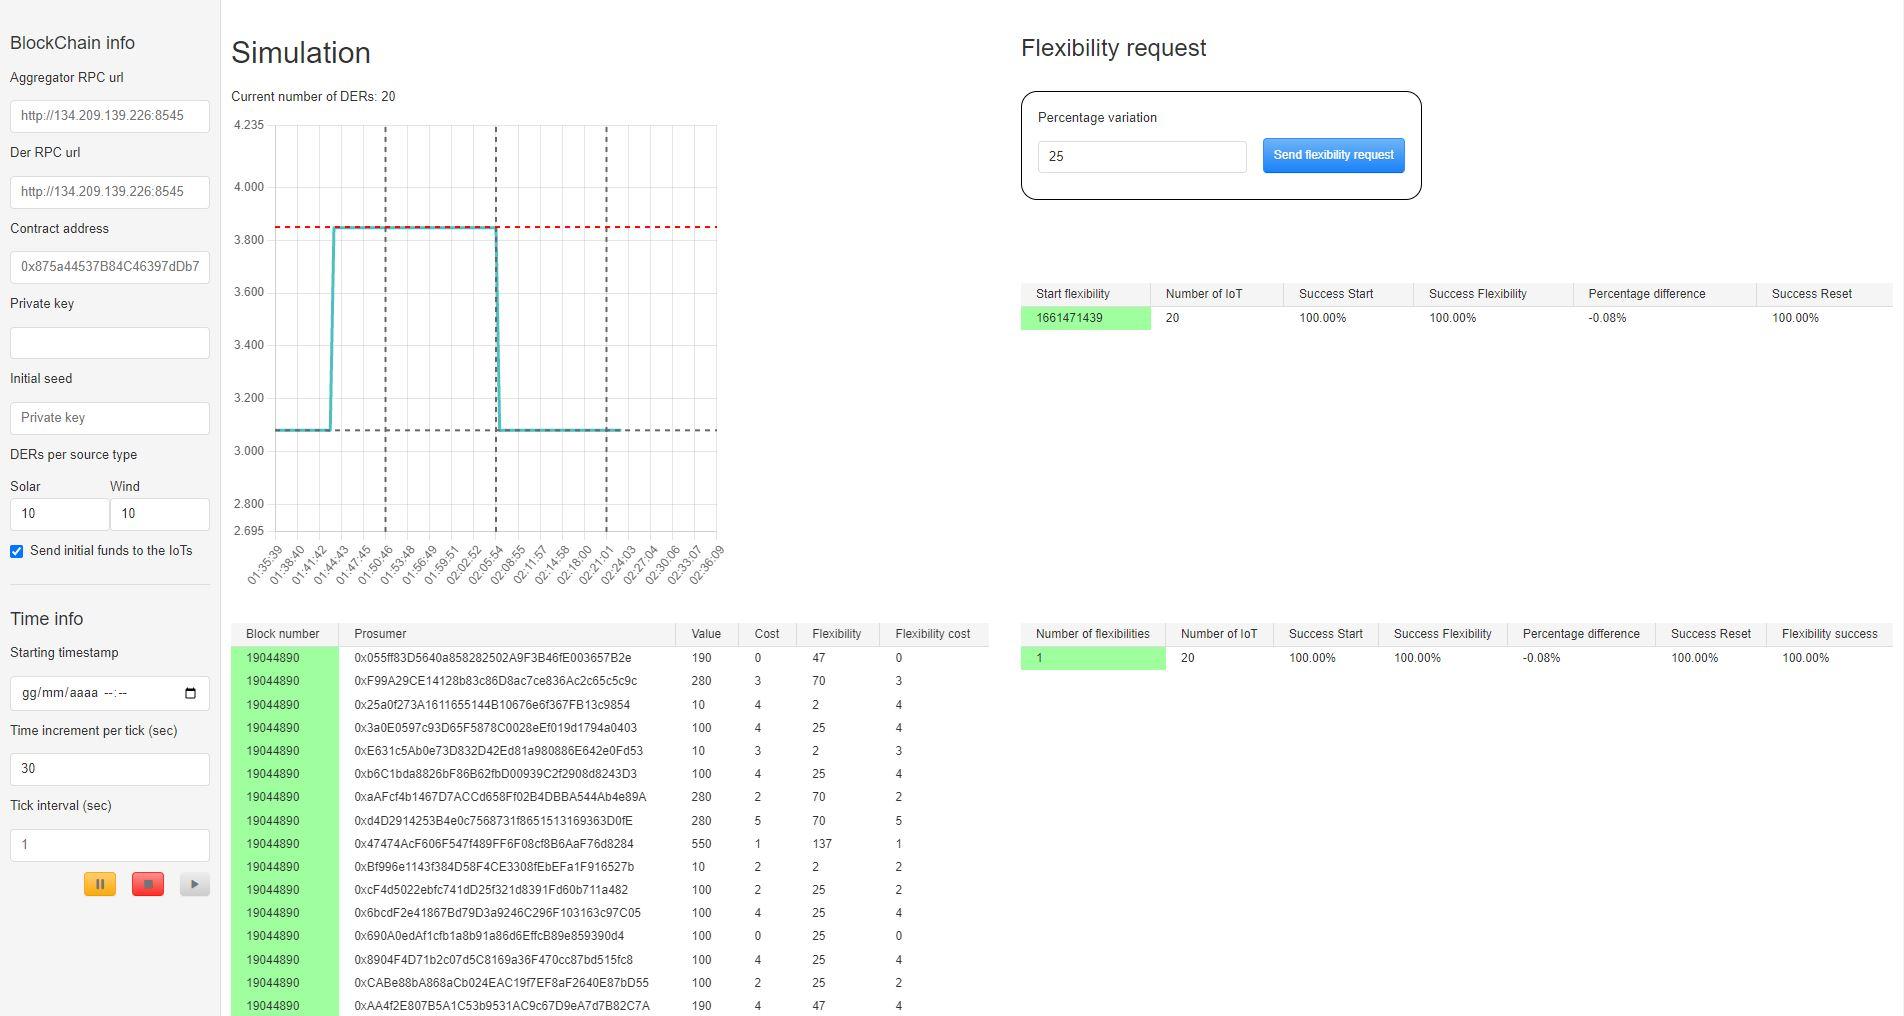
\includegraphics[width=\textwidth]{img/SimulatorFlexibility.jpg}
    \caption{Schermata del simulatore alla conclusione di un evento di flessibilità \label{fig:simulator-flexibility}}
\end{figure}